%%%%%%%% ICML 2019 submission %%%%%%%%%%%%%%%%%

\documentclass{article}
\renewcommand{\thesection}{\Alph{section}}
\renewcommand{\theequation}{A.\arabic{equation}}

\usepackage{microtype}
\usepackage{graphicx}
\usepackage[export]{adjustbox}
\usepackage{subcaption}
\usepackage{booktabs}
\usepackage{amsmath}
\usepackage{amsfonts, amsthm, amssymb}
\usepackage[parfill]{parskip}
\usepackage{enumerate}
\usepackage[shortlabels]{enumitem}
% \usepackage{hyperref}
\usepackage{bm}
\usepackage[colorlinks=true,citecolor=blue,urlcolor=blue,linkcolor=blue]{hyperref}
\usepackage{xr-hyper}
\usepackage{natbib}
\usepackage{fullpage}

\let\pprspace\relax
\externaldocument{arxiv_local_density_clustering}

\newcommand{\diam}{\mathrm{diam}}
\newcommand{\set}[1]{\left\{#1\right\}}
\newcommand{\defeq}{\overset{\mathrm{def}}{=}}
\newcommand{\vol}{\mathrm{vol}}
\newcommand{\abs}[1]{\left \lvert #1 \right \rvert}
\newcommand{\N}{\mathbb{N}}
\newcommand{\Reals}{\mathbb{R}}
\newcommand{\Rd}{\Reals^d}
\newcommand{\norm}[1]{\left\lVert#1\right\rVert}
\newcommand{\1}{\mathbf{1}}
\newcommand{\var}{\mathrm{Var}}
\newcommand{\Err}{\mathrm{Err}}
\newcommand{\Log}{\mathrm{Log}}
\newcommand{\TV}{\mathrm{TV}}
\newcommand{\dist}{\mathrm{dist}}
\newcommand{\Id}{\mathrm{Id}}

%%% Graph terms
\newcommand{\cut}{\mathrm{cut}}

%%% Vectors
\newcommand{\pbf}{\mathbf{p}}
\newcommand{\qbf}{\mathbf{q}}
\newcommand{\ebf}[1]{\mathbf{e}_{#1}}
\newcommand{\pibf}{\bm{\pi}}
\newcommand{\rhobf}{\bm{\rho}}
\newcommand{\Deltabf}{\bm{\Delta}}
\newcommand{\deltabf}{\bm{\delta}}
\newcommand{\zbf}{\mathbf{z}}

%%% Random walk vectors


%%% Matrices
\newcommand{\Abf}{\mathbf{A}}
\newcommand{\Xbf}{\mathbf{X}}
\newcommand{\Wbf}{\mathbf{W}}
\newcommand{\Lbf}{\mathbf{L}}
\newcommand{\Dbf}{\mathbf{D}}
\newcommand{\Ibf}[1]{\mathbf{I}_{#1}}

%%% Probability distributions (and related items)
\newcommand{\Pbb}{\mathbb{P}}
\newcommand{\Qbb}{\mathbb{Q}}
\newcommand{\Cbb}{\mathbb{C}}
\newcommand{\Ebb}{\mathbb{E}}

%%% Sets
\newcommand{\Sset}{\mathcal{S}}
\newcommand{\Cset}{\mathcal{C}}
\newcommand{\Aset}{\mathcal{A}}
\newcommand{\Asig}{\Aset_{\sigma}}
\newcommand{\Csig}{\Cset_{\sigma}}
\newcommand{\Asigr}{\Aset_{\sigma,\sigma + r}}
\newcommand{\Csigr}{\Cset_{\sigma,\sigma + r}}

%%% Operators
\DeclareMathOperator*{\argmin}{arg\,min}


%%% Algorithm notation
\newcommand{\ppr}{{\sc PPR}}
\newcommand{\pprspace}{{\sc PPR~}}

%%% Tilde notation for quantities over the expansion set 
\newcommand{\wn}{\widetilde{n}}
\newcommand{\wX}{\widetilde{\Xbf}}
\newcommand{\wx}{\widetilde{x}}
\newcommand{\wz}{\widetilde{z}}
\newcommand{\wbz}{\widetilde{\bf{z}}}
\newcommand{\wu}{\widetilde{u}}
\newcommand{\wPbb}{\widetilde{\Pbb}}
\newcommand{\wf}{\widetilde{f}}
\newcommand{\wDbf}{\widetilde{\Dbf}}


\newtheoremstyle{aldenthm}
{6pt} % Space above
{6pt} % Space below
{\itshape} % Body font
{} % Indent amount
{\bfseries} % Theorem head font
{.} % Punctuation after theorem head
{.5em} % Space after theorem head
{} % Theorem head spec (can be left empty, meaning `normal')

\theoremstyle{aldenthm}
\newtheorem{lemma}{Lemma}
\newtheorem{theorem}{Theorem}
\newtheorem{definition}{Definition}


%\newcommand{\theHalgorithm}{\arabic{algorithm}}


%\icmltitlerunning{Local clustering of density upper level sets}

\begin{document}

%\twocolumn[
%\icmltitle{Supplement to ``Local clustering of density upper level sets''}

%\icmlsetsymbol{equal}{*}

%\begin{icmlauthorlist}
%\icmlauthor{Alden Green}{cmu}
%\icmlauthor{Sivaraman Balakrishnan}{cmu}
%\icmlauthor{Ryan Tibshirani}{cmu}
%\end{icmlauthorlist}

%\icmlaffiliation{cmu}{Department of Statistics and Data Science, Carnegie Mellon University, Pittsburgh PA, USA}

%\icmlcorrespondingauthor{Alden Green}{ajgreen@andrew.cmu.edu}

%\icmlkeywords{local clustering}

%\vskip 0.3in
%]

%\printAffiliationsAndNotice{} % otherwise use the standard text.

\section{Proofs}

In this supplement, we present proofs for ``Local Clustering of Density Upper Level Sets''. Sections \ref{sec: volume_estimates} - \ref{sec: proof_of_theorem_1} detail the proof for Theorem \ref{thm: conductance_upper_bound}. \ref{sec: mixing_time_on_graphs} develops a bound of the form of \eqref{eqn: average_conductance}, which we recall links the conductance function to mixing time; this will be necessary for both Theorems \ref{thm: inverse_mixing_time_lower_bound_nonconvex} and \ref{thm: inverse_mixing_time_lower_bound}. \ref{sec: non_convex_conductance_function_and_local_spread} and \ref{sec: inverse_mixing_time_lower_bound_nonconvex} give the proof of Theorem \ref{thm: inverse_mixing_time_lower_bound_nonconvex}, while \ref{sec: convex_population_conductance_function}- \ref{sec: inverse_mixing_time_lower_bound} give the proof of Theorem \ref{thm: inverse_mixing_time_lower_bound}. \ref{sec: concentration} gives some general concentration results used throughout, before we finish with the proof of Theorem \ref{thm: consistent_recovery_of_density_clusters} in \ref{sec: proof_of_consistent_cluster_recovery}.

\subsection{Volume estimates}
\label{sec: volume_estimates}

Let $\Aset \subseteq \Reals^d$, and for $\sigma \geq 0$, write $\sigma B := B(0,\sigma) = \set{x \in \Rd: \norm{x} \leq \sigma}$ for the closed ball of radius $\sigma$ centered at the origin (and let $B^{\circ}(0,\sigma)$ denote the corresponding open ball). Let $\Asig = \Aset + \sigma B$ be the direct sum of $\Aset$ and $\sigma B$, $\Asig = \set{z = x + y: x \in \Aset, y \in \sigma B}$. 

\begin{lemma}
	\label{lem: expansion_volume}
	If $\Aset$ is closed and bounded, then for any $\delta > 0$,
	\begin{equation*}
	\nu(\Asig + \delta B) \leq \left(1 + \frac{\delta}{\sigma}\right)^d \nu(\Asig).
	\end{equation*}
\end{lemma}
\begin{proof}
	We will show that for any $\epsilon > 0$, 
	\begin{equation}
	\label{eqn: ratio_of_volume}
	\frac{\nu(\Asig + \delta B)}{\nu(\Asig)} \leq \frac{(\sigma + \delta + \epsilon)^d}{\sigma^d}
	\end{equation}
	which is sufficient to prove the claim.
	
	
	Fix $\epsilon > 0$. Our first goal is to find a finite collection $x_1, \ldots, x_N \in \Rd$ such that
	\begin{equation*}
	\bigcup_{i = 1}^{N} B(x_i, \sigma) \subseteq \Asig \subset \bigcup_{i = 1}^{N} B(x_i, \sigma + \epsilon). \tag{$N := N(\epsilon)$}
	\end{equation*}
	
	Observe that since $\Aset$ is closed and bounded, it is compact. As $B(x,\sigma)$ is compact, and the direct sum of two compact sets is itself compact, $\Asig$ is compact. Moreover,
	\begin{equation*}
	\Asig \subset \bigcup_{x \in \Aset} B^{\circ}(x,\sigma + \epsilon)
	\end{equation*}
	so by compactness there exists $x_1, \ldots,x_N \in \Aset$ such that
	\begin{equation*}
	\Asig \subset \bigcup_{i = 1}^{N} B^{\circ}(x_i,\sigma + \epsilon).
	\end{equation*}
	
	By the triangle inequality, $\Asig + \delta B \subset \bigcup_{i = 1}^{N} B^{\circ}(x_i,\sigma + \epsilon + \delta)$. Of course, for each $x_i \in \Aset$, $B(x_i,\sigma) \in \Asig$. Summarizing our findings, we have
	\begin{equation}
	\label{eqn: finite_subcover}
	\bigcup_{i = 1}^{N} B(x_i,\sigma) \subseteq \Asig  ,~\Asig + \delta B \subset \bigcup_{i = 1}^{N} B^{\circ}(x_i,\sigma + \delta + \epsilon)
	\end{equation}
	
	We next show a lower bound on $\nu(\Asig)$. Partition $\Asig$ using the balls $B(x_i,\sigma)$, meaning let $\Aset_{\sigma}^{(1)} := B(x_1,\sigma)$, $\Aset_{\sigma}^{(2)} := B(x_2,\sigma) \setminus B(x_1,\sigma)$, and continuing, so that
	\begin{equation*}
	\Aset_{\sigma}^{(i)} := B(x_i,\sigma) \setminus \bigcup_{j = 1}^{i - 1} \Aset_{\sigma}^{(j)}. \tag{$i = 1,\ldots,N$}
	\end{equation*}
	Observe that $\bigcup_{i = 1}^{N} \Asig^{(i)} = \bigcup_{i = 1}^{N} B(x_i,\sigma)$, so by \eqref{eqn: finite_subcover} $\Asig \supseteq \bigcup_{i = 1}^{N} \Asig^{(i)}$. As $\Asig^{(1)},\ldots, \Asig^{(N)}$ are non-overlapping,
	\begin{align*}
	\nu(\Asig) & \geq \sum_{i = 1}^{N} \nu(\Asig^{(i)}) \\
	& = \sigma^d \nu_d \sum_{i = 1}^{N}  \frac{\nu(\Asig^{(i)})}{\nu(B(x_i,\sigma))}
	\end{align*}
	We turn to proving an upper bound on $\nu(\Asig + \delta B)$. Let $\Aset_{\sigma + \epsilon + \delta}^{(1)} := B(x_1,\sigma + \delta + \epsilon)$ and
	\begin{equation*}
	\Aset_{\sigma + \delta + \epsilon}^{(i)} := B(x_i,\sigma + \delta + \epsilon) \setminus \bigcup_{j = 1}^{i - 1} \Aset_{\sigma + \delta + \epsilon}^{(j)}. \tag{$i = 2,\ldots,N$}
	\end{equation*}
	
	As $\bigcup_{i = 1}^{N} \Aset_{\sigma + \delta + \epsilon}^{(i)} = \bigcup_{i = 1}^{N} B(x_i,\sigma + \delta + \epsilon)$, by \eqref{eqn: finite_subcover}
	\begin{equation*}
	\Aset_{\sigma} + \delta B \subset \bigcup_{i =1}^{N} \Aset_{\sigma + \delta + \epsilon}^{(i)}
	\end{equation*}
	and therefore
	\begin{align*}
	\nu(\Aset_{\sigma + \delta}) & \leq \sum_{i = 1}^{N} \nu\bigl(\Aset_{\sigma + \delta + \epsilon}^{(i)}\bigr) \\
	& = \sum_{i = 1}^{N} \nu_d (\sigma + \delta + \epsilon)^d \frac{\nu(\Aset_{\sigma + \delta + \epsilon}^{(i)})}{\nu(B(x_i, \sigma + \delta + \epsilon))} \\
	& \leq \nu_d (\sigma + \delta + \epsilon)^d \sum_{i = 1}^{N} \frac{\nu(\Asig^{(i)})}{\nu(B(x_i,\sigma))}
	\end{align*}
	where the last inequality follows from Lemma \ref{lem: covering}. We have shown \eqref{eqn: ratio_of_volume}, and thus the claim.
\end{proof}

\begin{lemma}
	\label{lem: covering}
	For $i = 1, \ldots, N$ and  $A_{\sigma}^{(i)}, A_{\sigma + \delta + \epsilon}^{(i)}$ as in Theorem \ref{lem: expansion_volume},
	\begin{equation*}
	\frac{\nu(\Aset_{\sigma + \delta + \epsilon}^{(i)})}{\nu(B(x_i, \sigma + \delta + \epsilon))} \leq \frac{\nu(\Aset_{\sigma}^{(i)})}{\nu(B(x_i, \sigma))}
	\end{equation*}
\end{lemma}
\begin{proof}
	Let $\delta' := \delta + \epsilon$. It will be sufficient to show that
	\begin{equation*}
	\biggl(\Aset_{\sigma + \delta'}^{(i)} - \set{x_i}\biggr) \subseteq \left(1 + \frac{\delta'}{\sigma}\right)\cdot\biggl(\Asig^{(i)} - \set{x_i}\biggr) 
	\end{equation*}
	since then
	\begin{equation*}
	\nu(\Aset_{\sigma + \delta'}^{(i)}) \leq \left(1 + \frac{\delta'}{\sigma}\right)^d \nu(\Aset_{\sigma}^{(i)}) = \frac{\nu(B(x_i, \sigma + \delta'))}{\nu(B(x_i, \sigma))} \nu(\Aset_{\sigma}^{(i)}).
	\end{equation*}
	
	Assume without loss of generality that $x_i = 0$, and let $x \in \Aset_{\sigma + \delta'}^{(i)}$, meaning
	\begin{equation}
	\norm{x} \leq \sigma + \delta',~ \norm{x - x_j} > \sigma + \delta'~ \textrm{for $j = 1, \ldots, i - 1$}.
	\end{equation}
	Letting $x' = \frac{\sigma}{\sigma + \delta'} x$, since $\norm{x} \leq \sigma + \delta'$, $\norm{x'} \leq \sigma$ and therefore $x' \in B(0,\sigma)$. Additionally observe that for any $j = 1, \ldots, i - 1$, by the triangle inequality
	\begin{equation*}
	\norm{x' - x_j} \geq \norm{x - x_j} - \norm{x - x'} > \sigma + \delta' - \frac{\delta'}{\sigma + \delta'}\norm{x} \geq \sigma
	\end{equation*}
	and therefore $x' \not\in B(x_j,\sigma)$ for any $j = 1,\ldots, i - 1$. So $x' \in \Asig^{(i)}$.
\end{proof}

We will need to carefully control the volume of expansion sets using the estimate in Lemma \ref{lem: expansion_volume}; Lemma \ref{lem: Taylor_series} serves this purpose.
\begin{lemma}
	\label{lem: Taylor_series}
	For any $0 \leq x \leq 1/2d$,
	\begin{align*}
	(1 + x)^d & \leq 1 + 2dx \\
	(1 - x)^d & \geq 1 - 2dx.
	\end{align*}
\end{lemma}
\begin{proof}
	We take the binomial expansion of $(1 + x)^d$:
	\begin{align*}
	(1 + x)^d & = \sum_{k = 0}^{d} {d \choose k} x^k \\
	& = 1 + dx + dx\left(\sum_{k = 2}^d \frac{{d \choose k} x^{k - 1}}{d}\right)\\
	& \leq 1 + dx + dx\left(\sum_{k = 2}^d \frac{{d \choose k}}{(2d)^{k-1}d}\right) \tag{since $x \leq \frac{1}{2d}$} \\
	& \leq 1 + dx + dx\left(\sum_{k = 2}^d \frac{1}{2^{k - 1}}\right) \leq 1 + 2dx.
	\end{align*}
	
	The proof for the corresponding lower bound on $(1 - x)^d$ is symmetric.
\end{proof}

Let $\Csigr := \set{x: 0 < \dist(x, \Csig) < r}$, where $\Csig$ is as in Theorem \ref{thm: conductance_upper_bound}. Lemma \ref{lem: expected_number_boundary_points} involves the bulk of the technical effort required to prove Theorem \ref{thm: conductance_upper_bound}; it will be necessary to bound the expected cut size of $\Csig[\Xbf]$ in $G_{n,r}$. 

\begin{lemma}
	\label{lem: expected_number_boundary_points}
	Under the conditions of Theorem \ref{thm: conductance_upper_bound}, and for any $0 < r \leq \sigma/2d$,
	\begin{equation*}
	\Pbb(\Csigr) \leq \frac{2dr}{\sigma} \left(\lambda_{\sigma} - c_0\frac{r^{\gamma}}{\gamma + 1}\right) \nu(\Csig)
	\end{equation*}	
\end{lemma}
\begin{proof}
	We partition $\Csigr$ into slices based on distance from $\Csig$ as follows: for $k \in \N$,
	\begin{equation*}
	\mathcal{T}_{i,k} = \set{x \in \Csigr: t_{i,k} < \frac{\dist(x, \Csig)}{r} \leq t_{i+1,k}}, ~~ \Csigr = \bigcup_{i = 0}^{k-1} \mathcal{T}_{i,k}
	\end{equation*}
	where $t_i = i/k$ for $i = 0, \ldots, k - 1$. As a result, for any $k \in \mathbb{N}$,
	\begin{equation}
	\label{eqn: partition_ub}
	\Pbb(\Csigr) = \int_{\Csigr} f(x) dx = \sum_{i = 0}^{k-1} \int_{\mathcal{T}_{i,k}} f(x) dx \leq \sum_{i = 0}^{k-1} \nu(\mathcal{T}_{i,k}) \max_{x \in \mathcal{T}_{i,k}} f(x).
	\end{equation}
	
	\ref{asmp: bounded_density} and \ref{asmp: low_noise_density} imply the upper bound
	\begin{equation*}
	\max_{x \in \mathcal{T}_{i,k}} f(x) \leq \lambda_{\sigma} - c_0(rt_{i,k})^{\gamma},
	\end{equation*}
	and writing
	\begin{equation*}
	\nu(\mathcal{T}_{i,k}) = \nu(\Csig + rt_{i+1,k}B) - \nu(\Csig + rt_{i,k}B) =: \nu_{i+1,k} - \nu_{i,k},
	\end{equation*}
	we have
	\begin{align}
	\label{eqn: telescoping_sum}
	\sum_{i = 0}^{k-1} \nu(\mathcal{T}_{i,k}) \max_{x \in \mathcal{T}_{i,k}} f(x) & \leq \sum_{i = 0}^{k-1} \biggl\{ \nu_{i+1,k} - \nu_{i,k} \biggr\} \biggl( \lambda_{\sigma} - c_0(rt_{i,k})^{\gamma} \biggr) \nonumber \\
	& = \sum_{i = 1}^{k} 
	\underbrace{\nu_{i,k} \biggl( \left[\lambda_{\sigma} - c_0(rt_{i-1,k})^{\gamma}\right] -  \left[\lambda_{\sigma} - c_0(rt_{i,k})^{\gamma}\right]\biggr)}_{:= \Sigma_k} + \underbrace{\biggl(\nu_{k,k}\left[\lambda_{\sigma} - c_0r^{\gamma}\right] - \nu_{1,k}\lambda_{\sigma} \biggr)}_{:= \xi}
	\end{align}
	where the second equality comes from rearranging terms in the sum.
	
	We first consider the term $\Sigma_k$. $\Cset$ has finite diameter by \ref{asmp: cluster_diameter}. Letting $\overline{\Cset}$ be the closure of $\Cset$, we observe that $\overline{\Csig} = \overline{\Cset} + \sigma B$, and moreover for any $\delta > 0$, $\nu(\overline{\Csig} + \delta B) = \nu(\Csig + \delta B)$ (as $\partial(\Csig + \delta B)$ is Lipschitz and therefore has measure zero). As a result, for each $t_{i,k}, i = 1, \ldots,k$ we may apply Lemma \ref{lem: expansion_volume} to $\overline{\Cset}$ and obtain
	\begin{equation}
	\label{eqn: slice_volume_bound}
	\nu_{i,k} = \nu(\Csig + rt_{i,k}B) \leq \nu(\Csig)\left(1 + \frac{rt_{i,k}}{\sigma}\right)^d
	\end{equation}
	which in turn gives
	\begin{align}
	\Sigma_k & \leq c_0\nu(\Csig) r^\gamma \sum_{i = 1}^{k} \left(1 + \frac{ rt_{i,k}}{\sigma}\right)^d \biggl( (t_{i,k})^{\gamma} - (t_{i-1,k})^{\gamma}\biggr) \nonumber \\
	& = c_0\nu(\Csig) r^\gamma \sum_{i = 1}^{k} \left(1 + \frac{ru_{i,k}^{1/\gamma}}{\sigma}\right)^d ( u_{i,k} - u_{i,k-1}).~~~~~~~~~~~~~~ (u_{i,k} = t_{i,k}^{\gamma}) \label{eqn: Sigmak_riemann_sum}
	\end{align}
	\eqref{eqn: Sigmak_riemann_sum} is a Riemann sum, and taking the limit as $k \to \infty$ we obtain
	\begin{align}
	\lim_{k \to \infty} c_0\nu(\Csig) r^\gamma \sum_{i = 1}^{k} \left(1 + \frac{ru_{i,k}^{1/\gamma}}{\sigma}\right)^d ( u_{i,k} - u_{i,k-1}) & = c_0\nu(\Csig) r^\gamma \int_{0}^{1} \left(1 + \frac{r u^{1/\gamma}}{\sigma}\right)^{d} du \nonumber \\
	& \overset{(i)}{\leq} c_0\nu(\Csig) r^\gamma \int_{0}^{1} \left(1 + \frac{2 d r u^{1/\gamma}}{\sigma}\right) du \nonumber \\
	& = c_0\nu(\Csig) r^\gamma \left(1 + \gamma \frac{2 d r}{(\gamma + 1)\sigma}\right). \label{eqn: Sigmak_integral}
	\end{align}
	where $(i)$ follows from Lemma \ref{lem: Taylor_series} in light of the fact $r \leq \sigma / 2d$. 
	
	An upper bound on $\xi$ follows from largely the same logic, although it does not involve integration:
	\begin{align}
	\xi & \overset{(ii)}{\leq} \nu(\Csig) \biggl\{ \left(1 + \frac{ r}{\sigma}\right)^d(\lambda_{\sigma} - c_0r^{\gamma}) - \lambda_{\sigma} \biggr\} \nonumber \\
	& \overset{(iii)}{\leq} \nu(\Csig) \biggl\{ \left(1 + \frac{2d r}{\sigma}\right)(\lambda_{\sigma} - c_0r^{\gamma}) - \lambda_{\sigma} \biggr\} = \nu(\Csig) \biggl\{ \frac{2dr}{\sigma}(\lambda_{\sigma} - c_0r^{\gamma}) - c_0 r^{\gamma} \biggr\}. \label{eqn: xi_ub}
	\end{align}
	where $(ii)$ follows from \eqref{eqn: slice_volume_bound}, and $(iii)$ from Lemma \ref{lem: Taylor_series}. As the bounds in \eqref{eqn: partition_ub} and \eqref{eqn: telescoping_sum} hold for all $k$, these along with \eqref{eqn: Sigmak_integral} and \eqref{eqn: xi_ub} imply the desired result.
\end{proof}

Lemma \ref{lem: local_conductance} will be necessary to lower bound the expected volume of $\Csig[\Xbf]$ in $G_{n,r}$. Define the \emph{local conductance} $\ell_{\nu,r}(u)$ to be
\begin{equation*}
\ell_{\nu,r}(u) = \frac{\nu\left(\Csig \cap B(u,r)\right)}{\nu\left(B(u,r)\right)}.
\end{equation*}
\begin{lemma}
	\label{lem: local_conductance}
	Let $u \in \Csig$. Then, for any $0 < r \leq \frac{\sigma}{2\sqrt{d}}$,
	\begin{equation*}
	\ell_{\nu,r}(u) \geq \frac{6}{25}. 
	\end{equation*}
\end{lemma}
\begin{proof}
	Since $u \in \Csig$ there exists $x \in \Cset$ such that $u \in B(x, \sigma)$, and as $B(x,\sigma) \subseteq \Csig$,
	\begin{equation*}
	\nu\bigl(B(u, r) \cap B(x, \sigma)\bigr) \leq \nu\bigl(B(u, r) \cap \Csig \bigr).
	\end{equation*}
	Without loss of generality, let $\norm{u - x} = \sigma$; it is not hard to see that if $\norm{u - x} < \sigma$, the volume of the overlap will only grow. Then, since $\norm{u  - x} = \sigma$, $B(u, r) \cap B(x, \sigma)$ contains a spherical cap of radius $r$ and height
	\begin{equation*}
	h = r - (r)^2/2\sigma = r \left( 1 - \frac{r}{2 \sigma} \right)
	\end{equation*}	
	which by Lemma \ref{lem: volume_of_spherical_cap} has volume
	\begin{equation*}
	\nu_{cap} = \frac{1}{2} \nu_d r^d I_{1 - \alpha}\left( \frac{d + 1}{2}  ,\frac{1}{2}\right)
	\end{equation*}
	with $\alpha = 1 - \frac{2rh - h^2}{r^2} = \frac{r^2}{4 \sigma^2} \leq \frac{1}{8d}$. 
	
	Then by Lemmas \ref{lem: beta_integral} (applied with $t = 1$) and \ref{lem: beta_function},
	\begin{align*}
	I_{1 - \alpha}\left( \frac{d + 1}{2}  ,\frac{1}{2}\right) & \geq 1 - \frac{\Gamma\bigl(\frac{d}{2}+ 1\bigr)}{\Gamma\bigl(\frac{d + 1}{2}\bigr) \Gamma\bigl(\frac{1}{2}\bigr)} \frac{3}{2\sqrt{d}} \\
	& \geq 1 - \frac{3}{4}\sqrt{\frac{d+2}{\pi d}} \geq 1 - \frac{3}{4}\sqrt{\frac{3}{2 \pi}}.
	\end{align*}
\end{proof}

The following formula for the volume of the spherical cap, stated in terms of the incomplete beta function, is well known. We include it without proof. 

\begin{lemma}
	\label{lem: volume_of_spherical_cap}
	Let $\mathrm{Cap}_r(h)$ denote a spherical cap of radius $r$ and height $h$. Then, 
	\begin{equation*}
	\nu\bigl( \mathrm{Cap}_r(h)  \bigr) = \frac{1}{2} \nu_d r^d I_{1 - \alpha}(\frac{d + 1}{2}; \frac{1}{2})
	\end{equation*}
	where
	\begin{equation*}
	\alpha := 1 - \frac{2 r h - h^2}{r^2}
	\end{equation*}
	and
	\begin{equation*}
	I_{1 - \alpha}(z,w) = \frac{\Gamma(z + w)}{\Gamma(z) \Gamma(w)} \int_{0}^{1 - \alpha} u^{z - 1} (1 - u)^{w - 1} du.
	\end{equation*}
	is the cumulative distribution function of a $\mathrm{Beta}(z,w)$ distribution, evaluated at $1 - \alpha$. 
\end{lemma}

\begin{lemma}
	\label{lem: beta_integral}
	For any $0 \leq t \leq 1$ and $\alpha \leq \frac{t^2}{8 d}$,
	\begin{equation*}
	\int_{0}^{1 - \alpha}u^{(d-1)/2}(1 - u)^{-1/2}du \geq \frac{\Gamma\bigl(\frac{d + 1}{2}\bigr)\Gamma\bigl(\frac{1}{2}\bigr)}{ \Gamma\bigl(\frac{d}{2}+ 1\bigr)} - \frac{3t}{2\sqrt{d}}
	\end{equation*}
\end{lemma}
\begin{proof}
	We can write 
	\begin{equation*}
	\int_{0}^{1 - \alpha}u^{(d-1)/2}(1 - u)^{-1/2}du = \int_{0}^{1}u^{(d-1)/2}(1 - u)^{-1/2}du - \int_{1 - \alpha}^{1}u^{(d-1)/2}(1 - u)^{-1/2}du
	\end{equation*}
	The first integral is simply the beta function, with
	\begin{equation*}
	B(\frac{d+1}{2},\frac{1}{2}) := \frac{\Gamma\bigl(\frac{d + 1}{2}\bigr)\Gamma\bigl(\frac{1}{2}\bigr)}{ \Gamma\bigl(\frac{d}{2}+ 1\bigr)}.
	\end{equation*}
	To upper bound the second integral, we apply the Taylor theorem with remainder to $(1 - u)^{-1/2}$, obtaining
	\begin{equation*}
	(1 - u)^{-1/2} \leq \alpha^{-1/2} + \max_{u \in (1 - \alpha, 1)} \frac{\alpha}{2} (1 - u)^{-3/2} = \frac{3}{2}\alpha^{-1/2}.
	\end{equation*}
	As a result,
	\begin{align*}
	\int_{1 - \alpha}^{1}u^{(d-1)/2}(1 - u)^{-1/2}du & \leq \frac{3}{2}\alpha^{-1/2} \int_{1 - \alpha}^{1}u^{(d-1)/2}du \\
	& = \frac{3}{d+1}\alpha^{-1/2} \left(1 - (1 - \alpha)^{(d + 1)/2}\right) \\
	& \overset{(iv)}{\leq} \frac{3}{(d+1)}\alpha^{-1/2} (\alpha(d + 1)) \\
	& =  3\alpha^{1/2}.
	\end{align*}
	where $(iv)$ follows from Lemma \ref{lem: Taylor_series}, and the condition $\alpha \leq \frac{t^2}{8d}$. The result follows from the condition $\alpha \leq \frac{t^2}{8d}$. 
\end{proof}

Lemma \ref{lem: beta_function} follows from $\Gamma(1/2) = \sqrt{\pi}$ and the upper bound $\Gamma(x + 1)/ \Gamma(x+s) \leq (x + 1)^{1-s}$ for $s \in [0,1]$.
\begin{lemma}
	\label{lem: beta_function}
	\begin{equation*}
	\frac{\Gamma\bigl(\frac{d}{2}+ 1\bigr)}{\Gamma\bigl(\frac{d + 1}{2}\bigr) \Gamma\bigl(\frac{1}{2}\bigr)} \leq \sqrt{\frac{d + 2}{2\pi}}
	\end{equation*}
\end{lemma}

\subsection{Density-weighted cut and volume estimates}
\label{sec: density_weighted_cut_and_volume_estimates}

For notational ease, we write
\begin{align*}
\cut_{n,r} = \cut(\Csig[\Xbf]; G_{n,r}), ~ \mu_K = \mathbb{E}(\cut_{n,r}), ~ p_K = \frac{\mu_K}{{n \choose 2}} \\
\vol_{n,r} = \vol(\Csig[\Xbf]; G_{n,r}), ~ \mu_V = \mathbb{E}(\vol_{n,r}), ~ p_V = \frac{\mu_V}{{n \choose 2}} \\
\vol_{n,r}^c = \vol(\Xbf \setminus \Csig[\Xbf]; G_{n,r}), ~ \mu_V^c = \mathbb{E}(\vol_{n,r}^c), ~ p_V^c = \frac{\mu_V^c}{{n \choose 2}}
\end{align*}
for the random variable, mean, and probability of cut size and volume, respectively. 

\begin{lemma}
	\label{lem: expected_density_cut}
	Under the setup and conditions of Theorem \ref{thm: conductance_upper_bound}, and for any $0 < r \leq \sigma/2d$,
	\begin{equation*}
	p_K \leq \frac{4 d \nu_d r^{d+1} \lambda}{\sigma} \left(\lambda_{\sigma} - c_0\frac{r^{\gamma}}{\gamma + 1}\right) \nu(\Csig)
	\end{equation*}
\end{lemma}
\begin{proof}
	We can write $\cut_{n,r}$ as a double sum,
	\begin{equation}
	\label{eqn: density_cut_expansion}
	\cut_{n,r} = \sum_{i = 1}^{n} \sum_{j \neq i} \1(x_i \not\in \Csig) \1(x_j \in \Csig) \1(\norm{x_i - x_j} \leq r)
	\end{equation}
	and by linearity of expectation, we obtain
	\begin{equation*}
	p_K = \frac{\mu_K}{{n \choose 2}} = 2 \cdot \Pbb(x_i \not\in \Csig, x_j \in \Csig, \norm{x_i - x_j} \leq r). \tag{for each $i,j$, $i \neq j$}
	\end{equation*}
	Writing this with respect to the density function $f$, we have
	\begin{align*}
	p_K & = 2 \int_{\Rd \setminus \Csig} f(x) \Pbb\bigl(B(x,r) \cap \Csig\bigr) dx \\
	& = 2 \int_{\Csigr} f(x) \Pbb\bigl(B(x,r) \cap \Csig\bigr) dx \\
	& \leq 2 \nu_d r^d \lambda  \int_{\Csigr} f(x) dx = 2 \nu_d r^d \lambda \Pbb(\Csigr).
	\end{align*}
	where the inequality follows from \ref{asmp: cluster_separation}, which implies $f(x) \leq \lambda$ for $x \in \Csig \setminus \Cset$. Then, upper bounding the integral using Lemma \ref{lem: expected_density_cut} gives the final result.
\end{proof}

\begin{lemma}
	\label{lem: expected_density_volume}
	Under the setup and conditions of Theorem \ref{thm: conductance_upper_bound}, and for any $0 < r \leq \sigma/2d$,
	\begin{equation*}
	p_V \geq \frac{12}{25} \lambda_{\sigma}^2 \nu_d r^d \nu(\Csig)
	\end{equation*}
\end{lemma}
\begin{proof}
	The proof will proceed similarly to Lemma \ref{lem: expected_density_cut}. We begin by writing $\vol_{n,r}$ as the sum of indicator functions,
	\begin{equation}
	\label{eqn: volume_expansion}
	\vol_{n,r} = \sum_{i = 1}^{n} \sum_{j \neq i} \1(x_i \in \Csig) \1(x_j \in B(x_i, r))
	\end{equation}
	and by linearity of expectation we obtain
	\begin{equation*}
	p_V = \frac{\mu_V}{{n \choose 2}} = 2 \cdot \Pbb(x_i \in \Csig, x_j \in B(x_i,r)). \tag{for any $i,j$, $i \neq j$. }
	\end{equation*}
	Writing this with respect to the density function $f$, we have
	\begin{align*}
	p_V & = 2 \int_{\Csig} f(x) \Pbb(B(x,r)) dx \\
	& \geq 2 \int_{\Csig} f(x) \Pbb(B(x,r) \cap \Csig) dx
	\end{align*}
	whence the claim then follows by Lemma \ref{lem: local_conductance}.
\end{proof}

To employ Lemmas \ref{lem: expected_density_cut} and \ref{lem: expected_density_volume} in the proof of Theorem \ref{thm: conductance_upper_bound}, we must relate the random variable
\begin{equation*}
\Phi_{n,r}(\Csig[\Xbf]) = \frac{\cut_{n,r}}{\min \set{\vol_{n,r}, \vol_{n,r}^c}}
\end{equation*}
to $p_K$ and $p_V$. 

In Lemma \ref{lem: prob_bound_cutvol}, we give probabilistic bounds on the $\cut_{n,r}$, $\vol_{n,r}$ and $\vol_{n,r}^c$ in terms of $p_K$ and $p_V$. These bounds are a straightforward consequence of Lemma \ref{lem: bounded_difference}, Hoeffding's inequality for U-statistics.

\begin{lemma}
	\label{lem: prob_bound_cutvol}
	For any $\delta \in (0,1]$,
	\begin{equation}
	\label{eqn: numerator_additive_bound}
	\frac{\cut_{n,r}}{{n \choose 2}} \leq p_K + \sqrt{\frac{\log(1/\delta)}{n}},~\text{and}~ \frac{\vol_{n,r}}{{n \choose 2}}, \frac{\vol_{n,r}^c}{{n \choose 2}}  \geq p_V - \sqrt{\frac{\log(1/\delta)}{n}}.
	\end{equation}
	each with probability at least $1 - \delta$. 
\end{lemma}

\begin{proof}[Proof of Lemma \ref{lem: prob_bound_cutvol}]
	From \eqref{eqn: density_cut_expansion} and \eqref{eqn: volume_expansion}, we see that $\cut_{n,r}$ and $\vol_{n,r}$, properly scaled, can be expressed as order-$2$ $U$-statistics,
	\begin{equation*}
	\frac{\cut_{n,r}}{{n \choose 2}} = \frac{1}{{n \choose 2}} \sum_{1 \leq i < j \leq n} \phi_K(x_i, x_j),~~ \frac{\vol_{n,r}}{{n \choose 2}} = \frac{1}{{n \choose 2}} \sum_{1 \leq i < j \leq n} \phi_V(x_i, x_j)
	\end{equation*}
	with kernels
	\begin{align*}
	\phi_K(x_i,x_j) & = \1(x_i \in \Csig, x_j \not\in \Csig, \norm{x_i - x_j} \leq r) + \1(x_j \in \Csig, x_i \not\in \Csig, \norm{x_i - x_j} \leq r) \\
	\phi_V(x_i,x_j) & = \1(x_i \in \Csig, \norm{x_i - x_j} \leq r) + \1(x_j \in \Csig, \norm{x_i - x_j} \leq r). 
	\end{align*}
	
	Similarly,
	\begin{equation*}
	\frac{\vol_{n,r}^c}{{n \choose 2}} = \frac{1}{{n \choose 2}} \sum_{1 \leq i < j \leq n} \phi_{V^c}(x_i, x_j)
	\end{equation*}
	with kernel,
	\begin{equation*}
	\phi_{V^c}(x_i,x_j) = \1(x_i \not\in \Csig, \norm{x_i - x_j} \leq r) + \1(x_j \not\in \Csig, \norm{x_i - x_j} \leq r). 
	\end{equation*}
	
	From Lemma \ref{lem: bounded_difference} we therefore have
	\begin{equation*}
	\frac{\cut_{n,r}}{{n \choose 2}} \leq p_K + \sqrt{\frac{\log(1/\delta)}{n}},~  \frac{\vol_{n,r}}{{n \choose 2}} \geq p_V - \sqrt{\frac{\log(1/\delta)}{n}}, ~ \frac{\vol_{n,r}^c}{{n \choose 2}} \geq p_V^c - \sqrt{\frac{\log(1/\delta)}{n}}
	\end{equation*}
	each with probability at least $1 - \delta$. The claim follows in light of \eqref{eqn: weighted_cluster_volume}, which implies $p_V^c \geq p_V$. 
\end{proof}

\subsection{Proof of Theorem \ref{thm: conductance_upper_bound}}
\label{sec: proof_of_theorem_1}

The proof of Theorem \ref{thm: conductance_upper_bound} is more or less given by Lemmas \ref{lem: expected_density_cut}, \ref{lem: expected_density_volume}, and \ref{lem: prob_bound_cutvol}. All that remains is some algebra, which we take care of below.

Fix $\delta \in (0,1]$ and let $\delta' = \delta/3$. We rewrite
\begin{equation}
\label{eqn: conductance_representation_1}
\Phi_{n,r}(\Csig[\Xbf]) = \frac{p_K + \left(\frac{\cut_{n,r}}{{n \choose 2}} - p_K\right)}{p_V + \left(\frac{\min\set{\vol_{n,r}, \vol_{n,r}^c}}{{n \choose 2}} - p_V\right)}.
\end{equation}
Assume (\ref{eqn: numerator_additive_bound}) holds with respect to $\delta'$, keeping in mind that this will happen with probability at least $1 - \delta$. Along with (\ref{eqn: conductance_representation_1}) this means
\begin{equation*}
\Phi_{n,r}(\Csig[\mathbf{X}]) \leq \frac{p_K + \Err_n}{p_V - \Err_n}
\end{equation*}
for $\Err_n = \sqrt{\frac{\log(1/\delta')}{n}}$.
Now, some straightforward algebraic manipulations yield
\begin{align*}
\frac{p_K + \Err_n}{p_V - \Err_n} & = \frac{p_K}{p_V} \left(\frac{p_V}{p_V - \Err_n}\right) + \frac{\Err_n}{p_V - \Err_n} \\
& = \frac{p_K}{p_V} + \left(\frac{p_K}{p_V} + 1\right)\frac{\Err_n}{p_V - \Err_n} \\
& \leq \frac{p_K}{p_V} + 2 \frac{\Err_n}{p_V - \Err_n}.
\end{align*}
By Lemmas \ref{lem: expected_density_cut} and \ref{lem: expected_density_volume}, we have
\begin{equation*}
\frac{p_K}{p_V} \leq \frac{100rd}{12\sigma} \frac{\lambda}{\lambda_{\sigma}} \frac{\left(\lambda_{\sigma} - c_0\frac{r^{\gamma}}{\gamma + 1}\right)}{\lambda_{\sigma}}.
\end{equation*}
Then, by the choice of sample size in \eqref{eqn: conductance_sample_complexity}, 
\begin{equation*}
n \geq \frac{(2 + \epsilon)^2 \log\left(\frac{3}{\delta}\right)}{\epsilon^2 p_V^2}
\end{equation*}
which implies $2 \frac{\Err_n}{p_V - \Err_n} \leq \epsilon$. 

\subsection{Mixing time on graphs}
\label{sec: mixing_time_on_graphs}

For $N \in \mathbb{N}$ and a set $V$ of $N$ vertices, take $G = (V,E)$ to be an undirected and unweighted graph, with associated adjacency matrix $\Abf$, random walk matrix $\Wbf$, and stationary distribution $\pibf = (\pi_u)_{u \in V}$ where $\pi_v = \frac{\Dbf_{vv}}{\vol(V; G)}$. For $v \in V$, 
\begin{equation}
\label{eqn: random_walk}
q_{vu}^{(m)} = e_v\Wbf^m e_u, ~~ \qbf_{v}^{(m)} = \left(q_{vu}^{(m)}\right)_{u \in V}, ~~ \qbf_v = (\qbf^{(1)}_{v\cdot},\qbf^{(2)}_{v\cdot}, \ldots), 
\end{equation}
denote respectively the $m$-step transition probability, distribution, and sequence distributions of the random walk over $G$ originating at $v$. Letting $\qbf = (\qbf_v)_{v \in V}$, the relative pointwise mixing time is thus
\begin{equation*}
\tau_{\infty}(\qbf; G) := \tau_{\infty}(\qbf; G) = \min\set{m: \forall u,v \in V, \frac{\abs{q_{vu}^{(m)} - \pibf_u}}{\pibf_u} \leq 1/4} 
\end{equation*}
where we include the extra dependency on $\qbf$ as we will need to consider mixing of various random walks. 

Two key quantities relate the mixing time to the expansion of subsets $S$ of $V$. The \emph{local spread} is defined to be
\begin{equation*}
s(G) := \frac{9D_{\min}}{10}\pi_{\min} 
\end{equation*}
for $D_{\min} := \min_{v \in V} \Dbf_{vv}$ and $\pi_{\min} := D_{\min} / \vol(V; G)$.


%\inf \set{t: \forall S \subset V ~\text{with}~ \pi(S) = t, \beta(S) \leq 1/10}
%\end{equation*}
where $\beta(S) := \inf_{v \in S} \qbf_{v}^{(1)}(S^c)$, and by convention we let $\pbf(S) = \sum_{u \in S} p_u$ for any distribution vector $\pbf = (p_u)_{u \in V}$ over $V$. We collect some necessary facts about the local spread in Lemma \ref{lem: local_spread_G}.
\begin{lemma}
	\label{lem: local_spread_G}
	\begin{itemize}
		\item If $\pibf(S) \leq s(G)$, then for every $u \in S$, $\qbf_u^{(1)}(S^c) \geq 1/10$.
		\item For any $v, u \in V$, and $m \in N$ greater than $0$, $q_{vu}^{(m)}/ \pi_{\min} \leq 1/s(G)$.
	\end{itemize}
	
\end{lemma}

\begin{proof}
	If $t = \pibf(S) \leq \frac{9 D_{\min}}{10} \pi_{\min}$, divide both sides by $\pi_{\min}$ to obtain
	\begin{equation*}
	\abs{S} \leq \frac{9 D_{\min}}{10}
	\end{equation*}
	which implies $\qbf_{v}^{(1)}(S^c) \geq 1/10$ for all $v \in S$. This implies the first statement.
	
	The second statement follows from the fact $q_{vu}^{(m)} \leq 1/D_{\min}$ for any $m$.
\end{proof}

The local spread facilitates conversion between $\tau_{\infty}(\qbf_v; G)$ and the more easily manageable \emph{total variation} mixing time, given by
\begin{equation*}
\tau_1(\rhobf; G) = \min\biggl\{m: \forall v \in V, \norm{\rhobf_v - \pibf}_{TV} \leq 1/4 \biggr\}
\end{equation*}
where 
\begin{equation}
\label{eqn: uniform_random_walk}
\rhobf_{v}^{(m)} = \frac{1}{m}\sum_{k = 1}^{m+1} \qbf_{v}^{m}, ~~ \rhobf_v = \left( \rhobf_{v}^{(1)}, \rhobf_{v}^{(2)}, \rhobf_{v}^{(3)} \ldots \right), ~~ \rhobf = \left( \rhobf_v \right)_{v \in V}
\end{equation}
and $\norm{\pbf - \pibf}_{TV} = \sum_{v \in V}\abs{p_v - \pi_v}$ is the total variation norm between distributions $\pbf$ and $\pibf$. 
\begin{lemma}
	\label{lem: tv_mixing_to_pointwise_mixing1}
	For $\qbf$ as in \eqref{eqn: random_walk} and $\rhobf$ as in \eqref{eqn: uniform_random_walk},
	\begin{equation*}
	\tau_{\infty}(\qbf; G) \leq 2752 \tau_1(\rhobf; G) \log \left(4 \max\left\{1, \frac{1}{s(G)}\right\}\right)
	\end{equation*}
\end{lemma}
\begin{proof}
	Masking dependence on the starting vertex $v$ for the moment, let
	\begin{equation*}
	\Delta_u^{(m)} = q_{vu}^{(m)} - \pi_u, ~~ \delta_u^{(m)} = \frac{\Delta_u^{(m)}}{\pi_u}
	\end{equation*}
	and $\Deltabf^{(m)} = (\Delta_u^{(m)})_{u \in V}$, $\deltabf^{(m)} = (\delta_u^{(m)})_{u \in V}$. For a vector $\Deltabf = (\Delta_u)_{u \in V}$, the $L^{p}(\pibf)$ norm is given by
	\begin{equation*}
	\norm{\Deltabf}_{L^p(\pibf)} = \left(\sum_{u \in V} \left(\Delta_u\right)^{p} \pi_u \right)^{1/p}
	\end{equation*}
	To go between the $L^{\infty}(\pibf)$ and $L^{1}(\pibf)$ norms, we have
	\begin{align*}
	\norm{\deltabf^{(2m)}}_{L^{\infty}(\pi)} & \overset{(i)}{\leq} \norm{\deltabf^{(m)}}^2_{L^{2}(\pi)} \\
	& = \norm{(\deltabf^{(m)})^2}_{L^{1}(\pi)} \\
	& \overset{(ii)}{\leq}  \norm{(\deltabf^{(m)})}_{L^{1}(\pi)} \norm{(\deltabf^{(m)})}_{L^{\infty}(\pi)}
	\end{align*}
	where $(i)$ is a result of \cite{benjamini2003} and $(ii)$ follows from Holder's inequality. Now, we upper bound the second factor on the right hand side by observing
	\begin{align*}
	\norm{(\deltabf^{(m)})}_{L^{\infty}(\pi)} & \leq \max\left\{1, \max_{u \in V} \frac{q_{vu}^{(m)}}{\pi_u} \right\} \\
	& \overset{(iii)}{\leq} \max\left\{1, \frac{1}{s(G)}\right\}
	\end{align*}
	where $(iii)$ follows from Lemma \ref{lem: local_spread_G}.
	
	Now, we leverage the following well-known fact \cite{montenegro2002}: for any $\epsilon > 0$, if $m \geq \tau_1(\qbf_v^{(m)}; G) \cdot \log(1/\epsilon)$ then
	\begin{equation*}
	\norm{\qbf_v^{(m)} - \pibf}_{TV} \leq \epsilon.
	\end{equation*}
	But $\norm{\qbf_v^{(m)} - \pibf}_{TV}$ is exactly $\norm{(\deltabf^{(m)})}_{L^{1}(\pi)}$. Therefore, picking 
	\begin{equation*}
	m_0 = \tau_1(\qbf_v^{(m)}; G) \cdot \log \left(4 \max\left\{1, \frac{1}{s(G)}\right\} \right)
	\end{equation*} implies $\norm{(\deltabf^{(m)})}_{L^{\infty}(\pi)} \leq 1/4$ for all $m \geq 2 m_0$.  Then, 
	\begin{equation*}
	\norm{(\deltabf^{(m)})}_{L^{\infty}(\pi)} = \sup_{u}\left\{ \frac{\abs{q_{vu}^{(m)} - \pibf_u}}{\pibf_u} \right\}.
	\end{equation*}
	and since none of the above depended on a specific choice for $v$, the supremum can be taken over all starting vertices $v$ as well. Thus $\tau_{\infty}(\qbf^{(m)}; G) \leq 2m_0$. 
	
	Finally, it is known \cite{montenegro2002} that
	\begin{equation*}
	\tau_{1}(\qbf^{(m)}; G) \leq 1376 \tau_{1}(\rhobf^{(m)}; G)
	\end{equation*}
	and so the desired result holds.	
\end{proof}

The second key quantity is the \emph{conductance function}
\begin{equation}
\label{eqn: conductance_function}
\Phi(t; G) := \min_{\substack{S \subseteq V, \\ \pibf(S) \leq t} } \Phi(S; G) ~~~~~~~ (\pi_{\min} \leq t < 1)
\end{equation}
where $\Phi(S; G)$ is the normalized cut of $S$ in $G$ given by \eqref{eqn: norm_cut}. 

Lemma \ref{lem: expansion_to_tv_distance} leverages the conductance function and local spread to produce an upper bound on the total variation distance between $\rhobf_{v}^{(m)}$ and $\pibf.$
\begin{lemma}
	\label{lem: expansion_to_tv_distance}
	If $D_{\min} > 10$, for any $v \in V$:
	\begin{equation*}
	\norm{\rhobf_v^{(m)} - \pibf}_{TV} \leq \max\left\{ \frac{1}{4}, \frac{1}{10} +  \frac{70}{m}\left(\frac{20}{9} + \int_{t = s'(G)}^{1/2} \frac{4}{t \Phi^2(t; G)} dt\right) \right\}
	\end{equation*}
	where $s'(G) = s(G) / 9$.
\end{lemma}

To prove Lemma \ref{lem: expansion_to_tv_distance} we first introduce a generalization of $\Phi(t;G) \cdot \Phi(t;G)$ known as a blocking conductance function.
\footnote{For more details, see \cite{montenegro2002}}

\begin{definition}[Blocking Conductance Function of \cite{montenegro2002}]
	\label{def: blocking_conductance_function}
	For $t_0 \geq \pi_{\min}$, a function $\phi(t; G): [t_0, 1/2] \to [0,1]$ is a \emph{blocking conductance function} if for all $S \subset V$ with $\pibf(S) = t \in [t_0, 1/2]$, either of the following hold: 
	\begin{enumerate}
		\item \emph{Exterior inequality.} For all $y \in \left[\frac{1}{2}t, t\right]: \phi_{int}(S) \geq \phi(\max\{t_0,y\})$
		\item \emph{Interior inequality.} For all $y  \in \left[t, \frac{3}{2}t\right]: \phi_{ext}(S) \geq \phi(\max\{y,1 - y\})$.
	\end{enumerate}
	where $\phi_{int}$ and $\phi_{ext}$ are defined respectively as
	\begin{align*}
	\phi_{int}(S) & = \sup_{\lambda \leq \pibf(S)} \min_{\substack{B \subset S \\ \pibf(B) \leq \lambda} } \frac{\lambda \cut(S \setminus B, S^c; G)}{\vol(V; G) \left[\pibf(S) \pibf(S^c)\right]^2} \\
	\phi_{ext}(S) & = \sup_{\lambda \leq \pibf(S)} \min_{\substack{B \subset S^c \\ \pibf(B) \leq \lambda} } \frac{\lambda \cut(S \setminus B, S^c; G)}{\vol(V; G) \left[\pibf(S) \pibf(S^c)\right]^2}
	\end{align*}
\end{definition}

\begin{theorem}[Theorem 3.2 of \cite{montenegro2002}]
	\label{thm: montenegro}
	Consider $\phi(t; G): [t_0, 1/2] \to [0,1]$ a blocking conductance function. Then, letting
	\begin{equation*}
	h^m(t_0) = \sup_{S: \pibf(S) < t_0}  \bigl(\rhobf_v^{(m)}(S) - \pibf(S) \bigr)
	\end{equation*}
	the following statement holds: if $\phi$ is a blocking conductance function,
	\begin{align*}
	\norm{\rhobf_v^{(m)} - \pibf}_{TV} & \leq \max\left\{ \frac{1}{4}, h^1(t_0) +  \frac{70}{m}\left(\frac{1}{\phi(t_0; G)} + \int_{t = t_0}^{1/2} \frac{4}{t \phi(t; G)} dt\right) \right\} \\
	\end{align*}
\end{theorem}

Note that in \cite{montenegro2002} this theorem is stated with respect to $h^0$. However, in the subsequent proof it holds with respect to $h^m$, and it is observed that $h^m$ is decreasing in $m$. For our purposes it is more useful to state it with respect to $h^1$, as we have done.

\begin{proof}[Proof of Lemma \ref{lem:  expansion_to_tv_distance}]
	Consider the function $\phi_0(t, G): [s(G), 1/2] \to [0,1]$ defined by
	\begin{equation}
	\label{eqn: local_spread_blocking_conductance_function}
	\phi_0(t; G) = 
	\begin{cases}
	\frac{1}{5}, ~~~~~~~~~~~~ t = s'(G) \\
	\frac{1}{4} \Phi^2(t; G), ~ t \in \left(s'(G), 1/2\right] \\
	\end{cases}
	\end{equation}
	\begin{lemma}
		\label{lem: local_spread_blocking_conductance_function}
		If $D_{\min} > 10$, $\phi_0$ is a blocking conductance function.
	\end{lemma}
	We take Lemma \ref{lem: local_spread_blocking_conductance_function} as given, and defer the proof until after the proof of Lemma \ref{lem: expansion_to_tv_distance}. 
	
	Lemma \ref{lem: local_spread_blocking_conductance_function} and Theorem \ref{thm: montenegro} together yield:
	\begin{equation*}
	\norm{\rhobf^t - \pibf}_{TV} \leq \max\left\{ \frac{1}{4}, h^1(s'(G)) +  \frac{70}{m}\left(5 + \int_{t = s'(G)}^{1/2} \frac{4}{t \Phi^2(t; G)}\right) \right\}
	\end{equation*}
	
	Then, $h^1(s'(G)) \leq 1/10$ follows exactly from the proof of Lemma \ref{lem: local_spread_G}, except now $\pibf(S) \leq s'(G)$ results in the sharper bound of $\qbf_u^{(1)}(S^c) \geq 9/10$ for every $u \in S$.
\end{proof}
\begin{proof}[Lemma \ref{lem: local_spread_blocking_conductance_function}]
	The condition $D_{\min} > 10$ ensures that $s(G) \geq \pi_{\min}$.
	
	It is known that $\frac{1}{4} \Phi^2(x;G)$ satisfies the exterior inequality for all $t \in (\pi_{\min}, 1/2]$.
	
	For $t = s'(G)$ we will instead use the interior inequality. For any $S$ such that $\pibf(S) \leq s'(G)$, the following statement holds: for every $u \in S$, $\cut(u, S^c; G) \geq 9/10 \cdot \deg(u; G)$. 
	Fixing $\lambda = \pi(S)/2$, we have
	\begin{align*}
	\phi_{int}(S) & \geq \min_{\substack{B \subset S \\ \pibf(B) \leq \lambda} } \frac{\lambda \cut(S \setminus B, S^c; G)}{\vol(V; G) \left[\lambda (1 - \lambda)\right]^2} \\
	& \geq  \min_{\substack{B \subset S \\ \pibf(B) \leq \lambda} } \frac{9 \lambda \sum_{u \in S \setminus B} \deg(u; G)}{10 \vol(V; G) \left[\lambda (1 - \lambda)\right]^2} \\
	& \geq \frac{9\lambda^2}{20[\lambda^2(1 - \lambda)^2]} \geq \frac{9}{20}. 
	\end{align*} 
\end{proof}

\subsection{Conductance function and local spread: non-convex case.}
\label{sec: non_convex_conductance_function_and_local_spread}

We begin with some notation. Write $\Csig[\Xbf] = \wX$, and $G_{n,r}[\Csig[\Xbf]]$ as $\widetilde{G}_{n,r}$. For $S \subset \wX$, let $\widetilde{\cut}_{n,r}(S) = \cut(S;\widetilde{G}_{n,r})$ and similarly $\widetilde{\vol}_{n,r}(S) = \vol(S;\widetilde{G}_{n,r})$. 

Consider $\zbf \subset \Csig$ such that  $\mathcal{N}_{\zbf} = \set{B(z,r/3): z \in \zbf}$ is an internal covering of $\Csig$, meaning $\mathcal{N}_{\zbf} \supseteq \Csig$. Then, we write
\begin{align*}
\widetilde{B}_{\min} = \min_{z \in \zbf} \abs{B(z,r/3) \cap \wX}, ~~
\widetilde{D}_{\min} = \min_{\wx \in \wX} \abs{\widetilde{\cut}_{n,r}(x)} \\ \widetilde{B}_{\max} = \min_{z \in \zbf} \abs{B(z,r/3) \cap \wX}, ~~
\widetilde{D}_{\max} = \min_{\wx \in \wX} \abs{\widetilde{\cut}_{n,r}(x)}
\end{align*}
Both the conductance function and local spread will depend heavily on these quantities. Lemma \ref{lem: ball_bounds} collects the bounds we will need.
\begin{lemma}
	\label{lem: ball_bounds}
	Let $\Csig$ satisfy the conditions of Theorem \ref{thm: inverse_mixing_time_lower_bound_nonconvex}.	For sufficiently large $n$, and $r \leq \sigma/4d$, each of the following bounds hold with probability $1 - \delta$:
	\begin{align}
	\label{eqn: ball_bounds}
	\widetilde{B}_{\max} & \leq \left(1 + \sqrt{3^d\frac{3(\log \abs{\mathcal{N}_{\zbf}} + \log(1/\delta))}{n \nu_d r^d \Lambda_{\sigma}}}\right) n \nu_d \left(\frac{r}{3}\right)^d \Lambda_{\sigma} \nonumber \\
	\widetilde{B}_{\min} & \geq \left(1 - \sqrt{3^d\frac{2(\log \abs{\mathcal{N}_{\zbf}} + \log(1/\delta))}{n \nu_d r^d \lambda_{\sigma} \beta_d}}\right) n \nu_d \left(\frac{r}{3}\right)^d \lambda_{\sigma} \beta_d \nonumber \\
	\widetilde{D}_{\max} & \leq \left(1 + \sqrt{\frac{3(\log n + \log(1/\delta))}{n \nu_d r^d \Lambda_{\sigma}}}\right) n \nu_d r^d \Lambda_{\sigma} \nonumber \\
	\widetilde{D}_{\min} & \geq \left(1 - \sqrt{\frac{2(\log n + \log(1/\delta))}{n \nu_d r^d \lambda_{\sigma} \beta_d}}\right) n \nu_d \left(\frac{r}{3}\right)^d \lambda_{\sigma} \beta_d \nonumber \\
	\left(1 - \sqrt{\frac{2 \log(1/\delta)}{n \lambda_d \nu_d \sigma^d}}\right) n \lambda_{\sigma} \nu_d \sigma^d & \leq \widetilde{n} \leq \left(1 + \sqrt{\frac{3 \log(1/\delta)}{n \Lambda_{\sigma} \nu_d D^d}}\right) n \Lambda_d \nu_d D^d
	\end{align}
	where $\wn = \abs{\wX}$ and $\beta_d \geq 1/2^d$.
	
	In particular, fix $\epsilon > 0$. Then, for $n$ as specified in Theorem \ref{thm: inverse_mixing_time_lower_bound_nonconvex}, the following event:
	\begin{align}
	\label{eqn: ball_bounds_epsilon}
	\widetilde{B}_{\max} \leq \left(1 + \epsilon \right) n \nu_d \left(\frac{r}{3}\right)^d \Lambda_{\sigma},& ~~ \widetilde{D}_{\max} \leq \left(1 + \epsilon \right) n \nu_d r^d \Lambda_{\sigma} \nonumber \\
	\widetilde{B}_{\min} \geq \left(1 - \epsilon \right) n \nu_d \left(\frac{r}{3}\right)^d \lambda_{\sigma} \beta_{d},& ~~ \widetilde{D}_{\min} \geq \left(1 - \epsilon \right) n \nu_d r^d \lambda_{\sigma} \beta_{d} \nonumber \\
	(1 - \epsilon) n \lambda_{\sigma} \nu_d \sigma^d & \leq \widetilde{n} \leq (1 + \epsilon) n \Lambda_{\sigma} \nu_d D^d 
	\end{align}
	occurs with probability at least $1 - \delta$.
\end{lemma}
\begin{proof}
	We observe that for any $s \leq \sigma/4d$ and any $x \in \Csig$,
	\begin{equation*}
	\nu(B(x,s) \cap \Csig) \geq \left(\frac{s}{2}\right)^d = s^d \beta_d.
	\end{equation*}
	(In fact, tighter bounds can be shown to hold, but we will not need them). Therefore, by \ref{asmp: bounded_density}:
	\begin{equation*}
	\lambda_{\sigma} \nu_d s^d \beta_d \leq \Pbb\left(B(z,s) \cap \Csig \right) \leq \Lambda_{\sigma} \nu_d s^d \\
	\end{equation*}
	In particular, this holds for $s = r$ and $s = r/3$, and for every $z \in \zbf$ as well as every $z \in \widetilde{\Xbf}$. Now, by \ref{asmp: cluster_diameter} and \ref{asmp: bounded_density} we also have
	\begin{equation*}
	\Lambda_{\sigma} \nu_d \sigma^d \leq \Pbb(\Csig) \leq \Lambda_{\sigma} \nu_d D^d
	\end{equation*}
	
	The proof of each statement in \eqref{eqn: ball_bounds} then follows from application of Lemma \ref{lem: multiplicative_Hoeffding}. 
	
	To show \eqref{eqn: ball_bounds_epsilon}, we note that $\abs{\mathcal{N}_z}$ is less than the covering number of the $D$-ball in $d$ dimensions. Therefore
	\begin{equation*}
	\abs{\mathcal{N}_z} \leq \left(\frac{6D}{r} + 1\right)^d.
	\end{equation*}
	It is then immediately apparent that $n$ chosen as in Theorem \ref{thm: inverse_mixing_time_lower_bound_nonconvex} yields \eqref{eqn: ball_bounds_epsilon}.
\end{proof}

Now, we consider the conductance function and local spread computed over $\widetilde{G}_{n,r}$, which we refer to by
\begin{equation*}
\widetilde{\Phi}_{n,r}(t) = \Phi(t; \widetilde{G}_{n,r}), ~~ \widetilde{s}_{n,r} = s(\widetilde{G}_{n,r}).
\end{equation*}
where the restriction in the minimization problem of \eqref{eqn: conductance_function} is with respect to $\widetilde{\pi}_{n,r}$ the stationary distribution over $\widetilde{G}_{n,r}$.

We will bound $\widetilde{\Phi}_{n,r}(1/2)$ and $\widetilde{s}_{n,r}$ under the event that \eqref{eqn: ball_bounds_epsilon} holds, noting that this occurs with probability at least $1 - \delta$.

\begin{lemma}
	\label{lem: local_spread_lower_bound}
	If the bounds given by \eqref{eqn: ball_bounds_epsilon} hold, then
	\begin{equation*}
	\widetilde{s}_{n,r} \geq \frac{9}{10} \frac{(1 + \epsilon)^2}{(1 - \epsilon)^2}\frac{\lambda_{\sigma}^2}{\Lambda_{\sigma}^2} \frac{r^d}{D^d} \beta_d^2
	\end{equation*}
\end{lemma}

\begin{proof}
	The local spread can be written as
	\begin{equation*}
	\widetilde{s}_{n,r} = \frac{9}{10} \frac{\widetilde{D}_{\min}^2}{\widetilde{\vol}_{n,r}(\widetilde{G}_{n,r})} \geq  \frac{9}{10} \frac{\widetilde{D}_{\min}^2}{\widetilde{D}_{\max} \wn}.
	\end{equation*}
	Then apply the relevant results of Lemma \ref{lem: ball_bounds}.
\end{proof}

\begin{lemma}
	\label{lem: non_convex_conductance_lower_bound}
	If the bounds given by \eqref{eqn: ball_bounds_epsilon} hold, then:
	\begin{equation*}
	\widetilde{\Phi}_{n,r}(1/2) \geq \frac{\lambda_{\sigma}(1 - \epsilon)\beta_d}{4\Lambda_{\sigma}(1 + \epsilon)3^d} \left(1 + \frac{(1 - \epsilon)r^d\lambda_{\sigma}}{(1 + \epsilon)D^d\Lambda_{\sigma}}\right)
	\end{equation*}
\end{lemma}

\begin{proof}
	Fix $S \subset \wX$ with $\widetilde{\pi}_{n,r}(S) \leq 1/2$. Partition $\mathcal{N}_{\zbf} = \mathcal{N}_{\zbf}^+ \cup \mathcal{N}_{\zbf}^-$, where
	\begin{align*}
	\mathcal{N}_{\zbf}^- & = \set{B(z,r/3): 2 \Bigl\vert B(z,r/3) \cap S\Bigr\vert \leq \abs{B(z,r/3) \cap \wX} } \\
	\mathcal{N}_{\zbf}^+ & = \mathcal{N}_{\zbf} \setminus \mathcal{N}_{\zbf}^-
	\end{align*}
	and correspondingly $S^- = \mathcal{N}_{\zbf}^- \cap S$, $S^+ = \mathcal{N}_{\zbf}^+ \cap S$, so
	\begin{equation*}
	\frac{\widetilde{\cut}_{n,r}(S)}{\widetilde{\vol}_{n,r}(S)} = \frac{\widetilde{\cut}_{n,r}(S^-; \widetilde{G}_{n,r} \setminus S) + \widetilde{\cut}_{n,r}(S^+; \widetilde{G}_{n,r} \setminus S)}{\widetilde{\vol}_{n,r}(S^-) + \widetilde{\vol}_{n,r}(S^+)}.
	\end{equation*}
	It is immediately apparent that the following bounds hold for all $S \subset \wX$:
	\begin{align*}
	\widetilde{\cut}_{n,r}(S^-; \widetilde{G}_{n,r} \setminus S) & \geq \frac{\abs{S^-} \widetilde{B}_{\min}}{2}\\
	\widetilde{\vol}_{n,r}(S^-) & \leq \abs{S^-} \widetilde{D}_{\max} \\
	\widetilde{\vol}_{n,r}(S^+) & \leq \widetilde{\vol}_{n,r}(\widetilde{G}_{n,r}) \1(\abs{N_{\zbf}^+} > 0 )
	\end{align*}
	If moreover $\abs{N_{\zbf}^+} < \abs{N_{\zbf}}$, then 
	\begin{equation*}
	\widetilde{\cut}_{n,r}(S^+; \widetilde{G}_{n,r} \setminus S) \geq \frac{\widetilde{B}_{\min}^2}{4} \1(\abs{N_{\zbf}^+} > 0)
	\end{equation*}
	follows from the fact that the graph $H_{n,r} = (\zbf, E_H)$, with ($z_i, z_j) \in E_H$ if $\norm{z_i - z_j} \leq r/3$, is connected. As a result, if $\abs{N_{\zbf}^+} < \abs{N_{\zbf}}$ we have
	\begin{equation}
	\label{eqn: normalized_cut_1}
	\frac{\widetilde{\cut}_{n,r}(S)}{\widetilde{\vol}_{n,r}(S)} \geq \frac{ \widetilde{B}_{\min}}{4\widetilde{D}_{\max}} +  \frac{\widetilde{B}_{\min}^2}{8 \widetilde{\vol}_{n,r}(\widetilde{G}_{n,r})}
	\end{equation}
	using the inequality $2(A + B)/ (C + D) \geq A/C + B/D$ for $A,B,C,D$ non-negative.
	
	If, on the other hand , $\abs{\mathcal{N}_{\zbf}^+} = \mathcal{N}_{\zbf}$, then \eqref{eqn: normalized_cut_1} holds with respect to $S^c$. Then, because $\widetilde{\pi}_{n,r}(S) \leq 1/2$, 
	\begin{equation*}
	\frac{\widetilde{\cut}_{n,r}(S^c)}{\widetilde{\vol}_{n,r}(S^c)} \leq \frac{\widetilde{\cut}_{n,r}(S)}{\widetilde{\vol}_{n,r}(S)}
	\end{equation*}
	and so we get the exact statement of \eqref{eqn: normalized_cut_1}. Noting, as in the proof of Lemma \ref{lem: local_spread_lower_bound}, that  $\widetilde{\vol}_{n,r}(\widetilde{G}_{n,r}) \leq \wn \cdot \widetilde{D}_{\max}$, the relevant results of Lemma \ref{lem: ball_bounds} yield the desired inequality. 
\end{proof}

\subsection{Proof of Theorem \ref{thm: inverse_mixing_time_lower_bound_nonconvex}}
\label{sec: inverse_mixing_time_lower_bound_nonconvex}

Throughout this proof, we will condition on the events of Lemmas \ref{lem: local_spread_lower_bound} and \ref{lem: non_convex_conductance_lower_bound},
namely
\begin{align*}
\widetilde{s}_{n,r} & \geq \frac{9}{10} \frac{(1 + \epsilon)^2}{(1 - \epsilon)^2}\frac{\lambda_{\sigma}^2}{\Lambda_{\sigma}^2} \frac{r^d}{D^d} \beta_d^2 \\
\widetilde{\Phi}_{n,r}(1/2) & \geq \frac{\lambda_{\sigma}(1 - \epsilon)\beta_d}{4\Lambda_{\sigma}(1 + \epsilon)3^d} \left(1 + \frac{(1 - \epsilon)r^d\lambda_{\sigma}}{(1 + \epsilon)D^d\Lambda_{\sigma}}\right)
\end{align*}
noting that for $n$ as chosen in Theorem \ref{thm: inverse_mixing_time_lower_bound}, this will occur with probability at least $1 - \delta$ (by Lemma \ref{lem: ball_bounds}).

As a reminder, we write $\Csig[\Xbf] = \wX$, and $G_{n,r}[\Csig[\Xbf]]$ as $\widetilde{G}_{n,r}$. Fix arbitrary $v \in \wX$, and let
\begin{equation*}
\widetilde{\qbf}_n^{(m)} = e_v \Wbf_{\wX}^t, ~~ \widetilde{\qbf}_n = (\widetilde{q}_n^{(1)}, \widetilde{\qbf}_n^{(2)}, \ldots)
\end{equation*}
Our goal is to upper bound $\tau_{\infty}(\widetilde{\qbf}_n; \widetilde{G}_{n,r})$. (As we will see, this bound will hold over all such starting vertices $v \in \wX$.)

By Lemma \ref{lem: local_spread_G},
\begin{align*}
\tau_{\infty}(\widetilde{\qbf}_n; \widetilde{G}_{n,r}) & \leq 2752 \tau_{1}(\widetilde{\qbf}_n; \widetilde{G}_{n,r}) \max\left\{2, \log\left(\frac{4}{\widetilde{s}_{n,r}}\right) \right\} \nonumber \\
& \leq 2752 \tau_{1}(\widetilde{\qbf}_n; \widetilde{G}_{n,r}) \max\left\{2, d\log\left(\frac{8 D (1 + \epsilon)^2 \Lambda_{\sigma}^2}{r (1 - \epsilon)^2 \lambda_{\sigma}^2}\right) \right\}
\end{align*} 

We now upper bound $\tau_{1}(\widetilde{\qbf}_n; \widetilde{G}_{n,r})$.  From Lemma \ref{lem: expansion_to_tv_distance}, we have that
\begin{align}
\label{eqn: mixing_time_bound_on_neighborhood_graph_thm2}
\tau_{1}(\widetilde{\qbf}_n; \widetilde{G}_{n,r}) & \leq \frac{1400}{3}\left(5 + \int_{\widetilde{s}_{n,r}}^{1/2} \frac{4}{t\widetilde{\Phi}_{n,r}^2(t)} dt\right) \nonumber \\
& \leq \frac{1400}{3}\left(5 + \int_{ s_{\Pbb,r}}^{1/2} \frac{4}{t\widetilde{\Phi}_{n,r}^2(t)} dt \right)
\end{align}
where $s_{\Pbb,r} = \frac{9}{10} \frac{(1 + \epsilon)^2}{(1 - \epsilon)^2}\frac{\lambda_{\sigma}^2}{\Lambda_{\sigma}^2} \frac{r^d}{D^d} \beta_d^2$.(Since $r$ remains constant, for sufficiently large $n$ the lower bound on $\widetilde{D}_{\min}$ of Lemma \ref{lem: ball_bounds} will be at least $10$, and therefore Lemma \ref{lem: local_spread_blocking_conductance_function} holds.)

Now, we can upper bound the average conductance integral:
\begin{align*}
\int_{ s_{\Pbb,r}}^{1/2} \frac{4}{t\widetilde{\Phi}_{n,r}^2(t)} dt & \leq \int_{ s_{\Pbb,r}}^{1/2} \frac{4}{t\widetilde{\Phi}_{n,r}^2(1/2)} dt \\
& \leq 64\frac{9^d\Lambda_{\sigma}^2(1 + \epsilon)^2\beta_d^2}{\lambda_{\sigma}^2(1 - \epsilon)^2} \left(1 + \frac{(1 - \epsilon)r^d\lambda_{\sigma}}{(1 + \epsilon)D^d\Lambda_{\sigma}}\right)^{-2} \log s_{\Pbb,r}.
\end{align*}

Plugging this in to \eqref{eqn: mixing_time_bound_on_neighborhood_graph_thm2} gives the desired upper bound on $\tau_{\infty}(\widetilde{q}_n, \widetilde{G}_{n,r})$, which translates to the lower bound of \eqref{eqn: inverse_mixing_time_lower_bound}.

\subsection{Population-level conductance function: convex case.}
\label{sec: convex_population_conductance_function}

When $\Cset$ is convex, we will make use of the theory developed in \ref{sec: mixing_time_on_graphs} with respect to the conductance function $\Phi(t; G_{n,r}[\Csig(\Xbf)])$. First, however, we introduce a population-level analogue to $\Phi(t; G_{n,r}[\Csig(\Xbf)])$ over the set $\Csig$, which we denote $\widetilde{\Phi}_{\Pbb,r}$. (In general, we will adopt the convention of using $\widetilde{f}$ to denote functionals computed with respect to $\Csig$.)

For $\Sset \subset \Rd$
\begin{equation*}
\nu_{\Pbb}(\Sset) := \int_{\Sset} f(x) dx
\end{equation*} 
is the weighted volume.

The $r$-ball walk over $\Csig$ is a Markov chain. For $x \in \Csig$ and $\Sset, \Sset' \subset \Csig$, the transition probability is given by
\begin{equation*}
\widetilde{P}_{\Pbb, r}(x;\Sset) := \frac{\nu_\Pbb(\Sset \cap B(x,r))}{\nu_\Pbb(\Csig \cap B(x,r))}.
\end{equation*}
The stationary distribution $\pi_{\Pbb,r}$ thus satisfies
\begin{equation*}
\int_{\Csig}  \widetilde{P}_{\Pbb, r}(x;\Sset) d\pi_{\Pbb,r}(x) = \pi_{\Pbb,r}(\Sset)
\end{equation*}
for all $\Sset \in \Csig$. A simple calculation yields 
\begin{equation*}
\ell_{\Pbb,r}(x) := \nu_\Pbb(\Csig \cap B(x,r)) ~~~ \pi_{\Pbb,r}(\Sset) := \frac{1}{\int_{\Csig} f(x) \ell_{\Pbb,r}(x) dx} \int_{\Sset} f(x) \ell_{\Pbb,r}(x) dx,
\end{equation*}
and therefore the ergodic flow is
\begin{align*}
\widetilde{Q}_{\Pbb, r}(\Sset, \Sset') & := \int_{\Sset} d\pi_{\Pbb,r}(x) P_{\Pbb, r}(x;\Sset') dx \\
& =  \frac{1}{\int_{\Csig} f(x) \ell_{\Pbb,r}(x) dx} \int_{\Sset} f(x) \left(\int_{\Sset' \cap B(x,r)} f(x') dx' \right) dx
\end{align*}
The continuous conductance function is then
\begin{align*}
\widetilde{\Phi}_{\Pbb,r}(t) & := \min_{\substack{\Sset \subset \Csig, \\ \pi_{\Pbb,r}(\Sset) \leq t} } \frac{\widetilde{Q}_{\Pbb,r}(\Sset, \Csig \setminus \Sset)}{\pi_{\Pbb,r}(\Sset)} \\
& = \min_{\substack{\Sset \subset \Csig, \\ \pi_{\Pbb,r}(\Sset) \leq t} } \frac{\int_{\Sset} f(x) \left(\int_{(\Csig \setminus \Sset) \cap B(x,r)} f(x') dx' \right) dx}{\int_{\Sset} f(x) \left(\int_{\Csig \cap B(x,r)} f(x') dx' \right) dx}.
\end{align*}

For $m > 0$ and $0 < t_0 < t_1 < \ldots < t_m < 1$, denote the \emph{stepwise approximation to $g$} by $\bar{g}$, defined as
\begin{equation}
\label{eqn: stepwise_approximation}
\bar{g}(t) = g(t_i), ~~ \text{ for $t \in [t_{i-1}, t_i]$ }
\end{equation}
The stepwise approximation will be important to showing the consistency results of Section \ref{sec: pointwise_consistency_of_conductance_function} can be translated to a uniform bound. Lemma \ref{lem: stepwise_approximation} shows that the approximation will not overly degrade our estimates of the population-level conductance function.
\begin{lemma}
	\label{lem: stepwise_approximation}
	\begin{itemize}
		\item For any function $f$ monotone decreasing in $t$ on the interval $[t_0,t_m]$, $\bar{f}(t) \leq f(t)$ for all $t \in [t_0,t_m]$.
		\item Fix
		\begin{equation*}
		g(t) = \log\left(\frac{1}{t}\right) \text{ for $x \in [t_0, 1/2]$}
		\end{equation*}
		If for all $i$ in $1,\ldots,m$, $(t_i - t_{i - 1}) \leq t_0/2$, then $\bar{g}(t)\geq g(t) / 2$.
	\end{itemize}
\end{lemma}

\begin{proof}
	The first statement is immediately obvious, and we turn to proving the second. 
	
	The upper bound $g(t) \geq \bar{g}(t)$ follows immediately from the fact that $g(t)$ is a decreasing function along with the first statement.
	
	By the concavity of the $\log$ function, 
	\begin{equation*}
	\bar{g}(t) = \log\left(\frac{1}{t_i}\right) \geq \log\left(\frac{1}{t}\right) - \frac{(t_i - t)}{t}.
	\end{equation*}
	As a result,
	\begin{equation*}
	\bar{g}(t) - \frac{g(t)}{2} \geq \frac{\log\left(\frac{1}{t}\right)}{2} - \frac{(t_i - t)}{t} \geq 1/2 - 1/2 = 0.
	\end{equation*}
\end{proof}

The following theorem is found in \cite{kannan04}. It gives a bound population-level conductance function over convex bodies, when the density is uniform.
\begin{theorem}[Restatement of \cite{kannan04} Theorem 4.6]
	\label{thm: kannan}
	Let $K \subset \Rd$ be a convex body of diameter $D$. Then for any $\Sset \subset K$ with $\pi_{\nu,r}(\Sset) \leq 1/2$,
	\begin{equation}
	\label{eqn: kannan}
	\frac{Q_{\nu,r}(\Sset, \Csig \setminus \Sset)}{\pi_{\nu,r}(\Sset)} > \min\left\{\frac{1}{288\sqrt{d}},\frac{r}{81 \sqrt{d}D}\log\left(1 + \frac{1}{\pi_{\nu,r}(\Sset)}\right)\right\}.
	\end{equation}
\end{theorem}

\begin{lemma}
	\label{lem: continuous_conductance_lower_bound}
	Under the conditions on $\Csig$ given by Theorem \ref{thm: inverse_mixing_time_lower_bound}, the following bounds hold: 
	\begin{itemize}
		\item 
		for $0 < t < 1/2$,
		\begin{equation*}
		\widetilde{\Phi}_{\Pbb,r}(t) > \min\left\{\frac{1}{288\sqrt{d}},\frac{r}{81 \sqrt{d}D}\log\left(1 + \frac{\lambda_{\sigma}^2}{\Lambda_{\sigma}^2 t}\right)\right\} \cdot \frac{\lambda_{\sigma}^4}{\Lambda_{\sigma}^4}
		\end{equation*}
		\item
		Let
		\begin{equation*}
		M = \frac{2^{d+1}D^d \Lambda_{\sigma}^2}{r^d \lambda_{\sigma}^2}
		\end{equation*}
		and $t_i = (i + 1)/M$ for $i = 0, \ldots, m - 1$. Then, for $1/M < t < 1/2$
		\begin{equation*}
		\overline{\Phi}_{\Pbb,r}(t) > \min\left\{\frac{1}{288\sqrt{d}},\frac{r}{162 \sqrt{d}D}\Log\left( \frac{\Lambda_{\sigma}^2}{\lambda_{\sigma}^2 t}\right)\right\} \cdot \frac{\lambda_{\sigma}^4}{\Lambda_{\sigma}^4}
		\end{equation*}
		where $\overline{\Phi}_{\Pbb,r}(t)$ is defined as in \eqref{eqn: stepwise_approximation} with respect to $t_0, \ldots t_{M - 1}$, and $\Log(A/t) = \max\{\log(1 + 2A), \log(A/t)\}$.
	\end{itemize}
\end{lemma}
Before we prove Lemma \ref{lem: continuous_conductance_lower_bound}, note that the choice of $M$ is made to ensure $t_0$ is greater than the local spread of $G_{n,r}\left[\Csig[\Xbf]\right]$, as we will see in Section \ref{sec: convex_consistency}.
\begin{proof}[Proof of Lemma \ref{lem: continuous_conductance_lower_bound}]
	We note that
	\begin{equation*}
	\pi_{\Pbb,r}(S) \leq \pi_{\nu,r}(S) \cdot \frac{\Lambda_{\sigma}^2}{\lambda_{\sigma}^2}, ~~~ Q_{\Pbb,r}(\Sset, \Csig \setminus \Sset) \geq Q_{\nu,r}(\Sset, \Csig \setminus \Sset) \cdot \frac{\lambda_{\sigma}^2}{\Lambda_{\sigma}^2}
	\end{equation*}
	
	Plugging these estimates in to \eqref{eqn: kannan} gives
	\begin{equation*}
	\frac{Q_{\Pbb,r}(\Sset, \Csig \setminus \Sset)}{\pi_{\Pbb,r}(\Sset)} > \min\left\{\frac{1}{288\sqrt{d}},\frac{r}{81 \sqrt{d}D}\log\left(1 + \frac{\lambda_{\sigma}^2}{\Lambda_{\sigma}^2 \pi_{\Pbb,r}(\Sset)}\right)\right\} \cdot \frac{\lambda_{\sigma}^4}{\Lambda_{\sigma}^4}
	\end{equation*}
	and since the right hand side is decreasing in $\pi_{\Pbb,r}(\Sset)$, the desired lower bound holds on $\widetilde{\Phi}_{\Pbb,r}(t)$.  The bound on $\overline{\Phi}_{\Pbb,r}(t)$ then follows from  $\Log(A/t) \leq \log(1 + 1/t)$ for all $0 < t < 1/2$ and application of Lemma \ref{lem: stepwise_approximation}.
\end{proof}

\subsection{Consistency of local spread and conductance function: convex case.}
\label{sec: convex_consistency}

The introduction of the stepwise approximation allows us to make use of Lemma \ref{lem: consistency_of_conductance_function}, which gives us (pointwise) consistency of the discrete graph functionals $\widetilde{\Phi}_{n,r}(t)$ to the continuous functionals $\widetilde{\Phi}_{\Pbb,r}(t)$.

We use $\omega_r(1)$ to denote a term which goes to infinity as $r \to 0$, and likewise $o_r(1)$ to denote a term which goes to $0$ as $r \to 0$. 

\begin{lemma}
	\label{lem: consistency_of_conductance_function}
	Fix $0 < t < 1/2$. Under the conditions on $\Csig$ given by Theorem \ref{thm: inverse_mixing_time_lower_bound}, the following statement holds: with probability one, as $n \to \infty$,
	\begin{equation}
	\label{eqn: pointwise_consistency_of_conductance_function}
	\liminf_{n \to \infty} \widetilde{\Phi}_{n,r}(t) \geq \min\left\{\widetilde{\Phi}_{\Pbb,r}(t), c_d r \omega_r(1)\right\}
	\end{equation}
	where $c_d$ is a constant which may depend on the dimension $d$ (as well as the distribution $\Pbb$), but not $r$.
	
	As a consequence, for $M$ and $(t_i)_{i=0}^{M-1}$ defined as in Lemma \ref{lem: continuous_conductance_lower_bound}, we have that
	\begin{equation}
	\label{eqn: consistency_of_stepapprox_conductance_function}
	\liminf_{n \to \infty} \overline{\Phi}_{n,r}(t) \geq \min\left\{\overline{\Phi}_{\Pbb,r}(t), c_d r \omega_r(1)\right\}
	\end{equation}
\end{lemma}
We defer the proof of pointwise consistency to Section \ref{sec: pointwise_consistency_of_conductance_function}. For now, we show that \eqref{eqn: consistency_of_stepapprox_conductance_function} is immediately implied by \eqref{eqn: pointwise_consistency_of_conductance_function}.

\begin{proof}[Proof of \eqref{eqn: consistency_of_stepapprox_conductance_function}]
	We take as given that for any $0 < t < 1/2$,
	\begin{equation*}
	\liminf_{n \to \infty} \widetilde{\Phi}_{n,r}(t) \geq \widetilde{\Phi}_{\Pbb,r}(t).
	\end{equation*}
	In particular, for sufficiently large $n$ this will occur for each of $t_0, t_1, \ldots, t_m$ and therefore
	\begin{equation*}
	\liminf_{n \to \infty} \overline{\Phi}_{n,r} \geq \overline{\Phi}_{\Pbb,r}
	\end{equation*}
	uniformly over $[1/m,1/2]$.
\end{proof}

\subsection{Pointwise consistency of conductance function: convex case.}
\label{sec: pointwise_consistency_of_conductance_function}

We will rely heavily on results of \cite{garciatrillos16}, which prove the same result but consider only a pointwise result on $\widetilde{\Phi}_{n,r}(1/2)$ rather than over the entire conductance function.

Let $\wX = \Csig[\Xbf] = \set{\wx_1, \ldots, \wx_{\wn}}$, and $\wn = \abs{\wX}$. Then
\begin{equation*}
\widetilde{\Pbb}_n := \frac{1}{\wn} \sum_{\wx_i \in \wX} \delta_{\wx_i}
\end{equation*}
is the empirical distribution of $\wX$. Likewise, for $\Sset \subset \Csig$ let $\widetilde{\Pbb}$ be the conditional distribution $\Pbb(x \in S \vert x \in \Csig)$, given by
\begin{equation*}
\widetilde{\Pbb}(\Sset) := \frac{\nu_{\Pbb}(\Sset)}{\nu_{\Pbb}(\Csig)}.
\end{equation*}
A Borel map $T: \Csig \to \wX$ is a \emph{transportation map} between $\widetilde{\Pbb}$ and $\widetilde{\Pbb}_n$ if
\begin{equation*}
\widetilde{\Pbb}(\Sset) = \widetilde{\Pbb}_n(T(\Sset))
\end{equation*}
for all $\Sset \in \Csig$. 

\begin{lemma}[Proposition 5 of \cite{garciatrillos16}]
	There exists a sequence of transportation maps $(T_{\wn})$ from $\widetilde{\Pbb}$ and $\widetilde{\Pbb}_n$ such that
	\begin{equation*}
	\limsup_{\wn \to \infty} \frac{\wn^{1/d} \norm{\Id - T_{\wn}}_{\L^{\infty}(\widetilde{\Pbb})}}{(\log \wn)^{p_d} } \leq C
	\end{equation*}
	where $p_d = 1/d$ for $d \geq 3$ and $3/4$ if $d = 2$. 
\end{lemma}
These are referred to stagnating transportation maps. We refer the curious reader to \cite{garciatrillos16} for more details.

For $S \subset \wX$, we will denote $\vol(S; \widetilde{G}_{n,r})$ by $\widetilde{\vol}_{n,r}(S)$, and likewise $\cut(S; \widetilde{G}_{n,r})$ by $\widetilde{\cut}_{n,r}(S)$.

Consider a sequence of sets $(S_{\wn})_{\wn \in \mathbb{N}}$, with $u_{\wn} = \1_{S_{\wn}}$ the characteristic function of $S_{\wn}$. Similarly, for $\Sset \subset \Csig$ let $u = \1_{\Sset}$. 

\begin{definition}
	For a sequence $(u_{\wn}) \in L^1(\widetilde{\Pbb}_{\wn})$ and $u \in L^1(\widetilde{\Pbb})$, we say $(u_{\wn})$ converges $TL^1$ to $u$ if there exists a sequence of stagnating transportation maps $(T_{\wn})$ such that
	\begin{equation*}
	\int_{\Csig} \abs{u(x) - (u_{\wn}) \circ T_{\wn}(x)} d\widetilde{\Pbb}(x) \to 0
	\end{equation*}
	and denote it $u_{\wn} \overset{TL^1}{\to} u$.
\end{definition}

\begin{lemma}
	\label{lem: cut_convergence}
	If $(u_{\wn}) \overset{TL^1}{\to} u$, with probability one
	\begin{equation*}
	\lim_{n \to \infty} \frac{\widetilde{\cut}_{n,r}(S_{\wn})}{\wn^2} = \int_{\Sset} \wf(x) \left(\int_{(\Csig \setminus \Sset) \cap B(x,r)} \wf(x') dx' \right) dx
	\end{equation*}
	where $\wf$ is the density function of $\wPbb$ over $\Csig$.
\end{lemma}

\begin{proof}
	We note immediately that $n \to \infty$ implies $\wn \to \infty$ with probability one.
	
	Now, we can write
	\begin{align*}
	 \frac{\widetilde{\cut}_{n,r}(S_{\wn})}{\wn^2} & = \frac{1}{\wn^2} \sum_{i = 1}^{\wn} \sum_{j = 1}^{\wn} u_{\wn}(\wx_i) \bigl( 1 - u_{\wn}(\wx_j) \1(\norm{\wx_i - \wx_j} \leq r) \bigr)  \\
	& = \int_{\Csig} \left(\int_{\Csig \cap B(x,r)} u_{\wn}(x) \bigl( 1 - u_{\wn}(x') \bigr) d\wPbb_n(x') \right) d\wPbb_n(x) \\
	& = \int_{\Csig} \left(u_{\wn} \circ T_{\wn}(x)\right) \left(\int_{\Csig \cap B(T_{\wn}(x),r)}  \left(1 - u_{\wn} \circ T_{\wn}(x') \right) d\wPbb(x') \right) d\wPbb(x).
	\end{align*}
	
	Note that, for any $x \in \Csig$,
	\begin{align*}
	\lim_{n \to \infty} \nu\bigl(B(T_{\wn}(x),r) \setminus B(x,r)\bigr) & = 0 \\
	\lim_{n \to \infty} \nu\bigl(B(x,r) \setminus B(T_{\wn}(x),r)\bigr) & = 0.
	\end{align*}
	and therefore
	\begin{equation*}
	\lim_{n \to \infty} \int_{\Csig \cap B(T_{\wn}(x),r)} \left(1 - u_{\wn} \circ T_{\wn}(x') \right) d\wPbb(x') = \lim_{n \to \infty} \int_{\Csig \cap B(x,r)}  \left(1 - u_{\wn} \circ T_{\wn}(x')\right) d\wPbb(x').
	\end{equation*}
	An application of the bounded convergence theorem yields
	\begin{align*}
	& \lim_{n \to \infty} \int_{\Csig} \left(u_{\wn} \circ T_{\wn}(x)\right) \left(\int_{\Csig \cap B(T_{\wn}(x),r)}  \left(1 - u_{\wn} \circ T_{\wn}(x') \right) d\wPbb(x') \right) d\wPbb(x) = \nonumber \\
	& \lim_{n \to \infty} \int_{\Csig} \left(u_{\wn} \circ T_{\wn}(x)\right) \left(\int_{\Csig \cap B(x,r)}  \left( 1 - u_{\wn} \circ T_{\wn}(x') \right) d\wPbb(x') \right) d\wPbb(x).
	\end{align*}
	Letting
	\begin{align*}
	\mathcal{I}_n^1 & = \int_{\Csig} \left(u(x)\right) \left(\int_{\Csig \cap B(x,r)}  \left( u(x') - u_{\wn} \circ T_{\wn}(x') \right) d\wPbb(x') \right) d\wPbb(x) \\
	\mathcal{I}_n^2 & = \int_{\Csig} \left(u_{\wn} \circ T_{\wn}(x) - u(x)\right) \left(\int_{\Csig \cap B(x,r)}  \left(1 - u_{\wn} \circ T_{\wn}(x') \right) d\wPbb(x') \right) d\wPbb(x) \\
	\end{align*}
	we have
	\begin{align}
	\label{eqn: pointwise_convergence_1}
	& \int_{\Csig} \left(u_{\wn} \circ T_{\wn}(x)\right) \left(\int_{\Csig \cap B(x,r)}  \left( 1 - u_{\wn} \circ T_{\wn}(x') \right) d\wPbb(x') \right) d\wPbb(x) = \nonumber \\
	& \int_{\Csig} u(x) \left\{ \int_{\Csig \cap B(x,r)} (1 - u(x')) d\wPbb(x') \right\} d\wPbb(x) + \mathcal{I}_n^1 + \mathcal{I}_n^2. 
	\end{align}
	
	Recalling that $u = 1_{\Sset}$, we can see
	\begin{align}
	\label{eqn: pointwise_convergence_2}
	\int_{\Csig} u(x) \left\{ \int_{\Csig \cap B(x,r)} (1 - u(x')) d\wPbb(x') \right\} d\wPbb(x) & = \int_{\Sset} \wf(x) \left(\int_{(\Csig \setminus \Sset) \cap B(x,r)} \wf(x') dx' \right) dx
	\end{align}
	Since $(u_{\wn}) \overset{TL^1}{\to} u$, another application of the bounded convergence theorem yields $\lim_{n \to \infty} \mathcal{I}_n^1 = \lim_{n \to \infty} \mathcal{I}_n^2 = 0$. Therefore by \eqref{eqn: pointwise_convergence_1} and \eqref{eqn: pointwise_convergence_2} the final result holds.
\end{proof}

\begin{lemma}
	\label{lem: vol_convergence}
	If $u_{\wn} \overset{TL^1}{\to} u$, then
	\begin{equation*}
	\lim_{n \to \infty} \frac{\widetilde{\vol}_{n,r}(S_{\wn})}{\wn^2} = 
	\int_{\Sset} \wf(x) \left(\int_{\Csig \cap B(x,r)} \wf(x') dx' \right) dx
	\end{equation*}
	with probability one. 
\end{lemma}
\begin{proof}
	We note that
	\begin{align*}
	\frac{\widetilde{\vol}_{n,r}(S_{\wn})}{\wn^2} & = \frac{1}{\widetilde{n}^2} \sum_{i = 1}^{\wn} \sum_{j = 1}^{\wn} u_{\wn}(\wx_i) \1(\norm{\wx_i - \wx_j} \leq r) - \frac{1}{\widetilde{n}} \\
	& = \int_{\Csig} \int_{\Csig \cap B(x,r)} \left(u_{\wn}(x) d\wPbb_n(x')\right) d{\wPbb}(x) - \frac{1}{\wn}
	\end{align*}
	Of course, $\lim_{n \to \infty}  \frac{1}{\wn} = 0$, and so
	\begin{equation*}
	\lim_{n \to \infty} \frac{\widetilde{\vol}_{n,r}(S_{\wn})}{\wn^2} = \lim_{n \to \infty} \int_{\Csig} \left(\Csig \cap B(x,r) u_{\wn}(x) d\wPbb_n(x')\right) d_{\wPbb}(x)
	\end{equation*}
	The proof then proceeds analogously to Lemma \ref{lem: cut_convergence}. 
\end{proof}

Lemma \ref{lem: pre-compactness} can be found in \cite{alberti1998non} (Theorem 3.1) or \cite{garciatrillos16} (Lemma 23).
\begin{lemma}
	\label{lem: pre-compactness}
	If $u_{\wn} \not\overset{TL^1}{\to} u$ for some $u \in L^1{\nu}$, with probability one:
	\begin{equation*}
	\liminf_{n \to \infty} \frac{\widetilde{\cut}_{n,r}(\Sset_{\wn})}{\wn^2 } \geq  c_d r^{d+1} \omega_r(1)
	\end{equation*}
	where $c_d$ is a constant which does not depend on $r$ but may depend on $\Csig$ and $f$, and $\omega_r(1) \to \infty$ as $r \to 0$. 
\end{lemma}

\begin{proof}[Proof of \eqref{eqn: pointwise_consistency_of_conductance_function}]
	Let $(S_{\wn}^{\star})$
	\begin{equation*}
	\frac{\widetilde{\cut}_{n,r}(S_{\wn}^{\star})}{\widetilde{\vol}_{n,r}(S_{\wn}^{\star})} = \widetilde{\Phi}_{n,r}(t),~~ \widetilde{\pi}_{n,r}(S_{\wn}) \leq t
	\end{equation*}
	be the sequence of minimizers of the normalized cut with stationary distribution at most $t$ in the graph $\widetilde{G}_{n,r}$. Denote $u_{\wn}^{\star} = 1_{S_{\wn}^{\star}}$, and assume that $u_{\wn}^{\star} \overset{TL^1}{\to} u$, for $u = 1_{\Sset}, ~\Sset \subset \Csig$. 
	Then, by Lemmas \ref{lem: cut_convergence} and \ref{lem: vol_convergence},
	\begin{align*}
	\lim_{n \to \infty} \frac{\widetilde{\cut}_{n,r}(S_{\wn})}{\widetilde{\vol}_{n,r}(S_{\wn})} & = \frac{\int_{\Sset} \wf(x) \left(\int_{(\Csig \setminus \Sset) \cap B(x,r)} \wf(x') dx' \right) dx}{\int_{\Sset} \wf(x) \left(\int_{\Csig \cap B(x,r)} \wf(x') dx' \right) dx} \\
	& \overset{(i)}{=} \frac{\int_{\Sset} f(x) \left(\int_{(\Csig \setminus \Sset) \cap B(x,r)} f(x') dx' \right) dx}{\int_{\Sset} f(x) \left(\int_{\Csig \cap B(x,r)} f(x') dx' \right) dx} 
	& = \frac{\widetilde{Q}_{\Pbb,r}(\Sset, \Csig \setminus \Sset)}{\pi_{\Pbb,r}(\Sset)}.
	\end{align*}
	where $(i)$ holds because the normalization factors present in $\wf$ cancel. From Lemma \ref{lem: vol_convergence}, we also have that $\lim_{n \to \infty}\widetilde{\pi}_{n,r}(S_{\wn}) = \pi_{\Pbb,r}(\Sset)$, and therefore $\pi_{\Pbb,r}(\Sset) \leq t$. As a result,
	\begin{equation*}
	\liminf_{n \to \infty} \widetilde{\Phi}_{n,r}(t) = \frac{\widetilde{Q}_{\Pbb,r}(\Sset, \Csig \setminus \Sset)}{\pi_{\Pbb,r}(\Sset)} \geq \widetilde{\Phi}_{\Pbb,r}(t).
	\end{equation*}
	On the other hand, if $u_{\wn}^{\star}$ does not converge $TL^1$, then
	\begin{equation*}
	\frac{\widetilde{\cut}_{n,r}(S_{\wn})}{\wn^2} \geq c_d r^{d+1} \omega_r(1)
	\end{equation*}
	Additionally,
	\begin{equation*}
	\frac{\widetilde{\vol}_{n,r}(S_{\wn})}{\wn^2} \leq \frac{\widetilde{\vol}_{n,r}(\widetilde{G}_{n,r})}{\wn^2}
	\end{equation*}
	and
	\begin{equation*}
	\limsup_{n \to \infty} \frac{\widetilde{\vol}_{n,r}(\widetilde{G}_{n,r})}{\wn^2} \leq \nu_d r^d \Lambda_{\sigma}
	\end{equation*}
	As a result,
	\begin{equation*}
	\liminf_{n \to \infty} \frac{\widetilde{\cut}_{n,r}(S_{\wn})}{\widetilde{\vol}_{n,r}(S_{\wn})} \geq c_d r \omega_r(1).
	\end{equation*}
\end{proof}

\subsection{Proof of Theorem \ref{thm: inverse_mixing_time_lower_bound}}
\label{sec: inverse_mixing_time_lower_bound}
Throughout this proof, we will refer to the subgraph $G_{n,r}\left[\Csig[\Xbf]\right]$ as $\widetilde{G}_{n,r}$. 

Fix arbitrary $v = x_i \in \Csig[\Xbf]$, and let
\begin{equation*}
\widetilde{\qbf}_n^{(m)} = e_v \Wbf_{\Csig[\Xbf]}^t, ~~ \widetilde{\qbf}_n = (\widetilde{q}_n^{(1)}, \widetilde{q}_n^{(2)}, \ldots)
\end{equation*}
Our goal is to upper bound $\tau_{\infty}(\widetilde{\qbf}_n; \widetilde{G}_{n,r})$.

By Lemmas \ref{lem: local_spread_G} and \ref{lem: local_spread_lower_bound},
\begin{align*}
\tau_{\infty}(\widetilde{\qbf}_n; \widetilde{G}_{n,r}) & \leq 2752 \tau_{1}(\widetilde{\qbf}_n; \widetilde{G}_{n,r}) \max\left\{2, \log\left(\frac{4}{\widetilde{s}_{n,r}}\right) \right\} \nonumber \\
& \leq 2752 \tau_{1}(\widetilde{\qbf}_n; \widetilde{G}_{n,r}) \max\left\{2, 4d\log\left(\frac{2D \Lambda_{\sigma}^2}{\lambda_{\sigma}^2}\right) \right\}
\end{align*} 

We now upper bound $\tau_{1}(\widetilde{\qbf}_n; \widetilde{G}_{n,r})$.  From Lemma \ref{lem: expansion_to_tv_distance}, we have that
\begin{equation}
\label{eqn: mixing_time_bound_on_neighborhood_graph}
\limsup_{n \to \infty} \tau_{1}(\widetilde{\qbf}_n; \widetilde{G}_{n,r}) \leq \limsup_{n \to \infty} \frac{1400}{3}\left(5 + \int_{\widetilde{s}_{n,r}}^{1/2} \frac{4}{t\widetilde{\Phi}_{n,r}^2(t)} dt\right)
\end{equation}
(Since $r$ remains constant, for sufficiently large $n$, $\Dbf_{xx} > C$ will be fulfilled for any $x \in \Csig[\Xbf]$, and any $C < \infty$.)
We set aside the constant term for the moment and turn to the integral. By Lemma \ref{lem: local_spread_lower_bound},
\begin{equation*}
\limsup_{n \to \infty}\int_{\widetilde{s}_{n,r}}^{1/2} \frac{4}{t\widetilde{\Phi}_{n,r}^2(t)} dt \leq \limsup_{n \to \infty}\int_{ s_{\Pbb,r}}^{1/2} \frac{4}{t\widetilde{\Phi}_{n,r}^2(t)} dt
\end{equation*}
where $s_{\Pbb,r}$ is as in the proof of Theorem \ref{thm: inverse_mixing_time_lower_bound_nonconvex}. We now replace the discrete conductance function $\widetilde{\Phi}_{n,r}$ by the stepwise approximation to the continuous conductance function, $\overline{\Phi}_{n,r}$:
\begin{align*}
\limsup_{n \to \infty}\int_{s_{\Pbb,r}}^{1/2} \frac{4}{t\widetilde{\Phi}_{n,r}^2(t)} dt & \overset{(i)}{\leq} \limsup_{n \to \infty}\int_{s_{\Pbb,r}}^{1/2} \frac{4}{t\overline{\Phi}_{n,r}^2(t)} dt \\
& = \int_{s_{\Pbb,r}}^{1/2} \limsup_{n \to \infty} \frac{4}{t\overline{\Phi}_{n,r}^2(t)} dt\\
& \overset{(ii)}{\leq} \int_{s_{\Pbb,r}}^{1/2} \frac{4}{t\overline{\Phi}_{\Pbb,r}^2(t)} dt + c_d^2 \log(s_{\Pbb,r}) \frac{1}{r^2} o_r(1)\\
\end{align*}
where $(i)$ follows from Lemma \ref{lem: stepwise_approximation} and $(ii)$ from Lemma \ref{lem: consistency_of_conductance_function} (along with the continuous mapping theorem). Now, we make use of Lemma \ref{lem: continuous_conductance_lower_bound}:
\begin{align*}
& \int_{s_{\Pbb,r}}^{1/2} \frac{4}{t\overline{\Phi}_{\Pbb,r}^2(t)} dt \leq \frac{\Lambda_{\sigma}^8}{\lambda_{\sigma}^8} \cdot \left( 331776
\int_{s_{\Pbb,r}}^{1/2} \frac{d}{t} dt + \int_{s_{\Pbb,r}}^{1/2} \frac{81dD^2}{r^2t \Log(\frac{\Lambda_{\sigma}^2}{t\lambda_{\sigma}^2})}  dt\right) \\
& \leq \frac{\Lambda_{\sigma}^8}{\lambda_{\sigma}^8} \cdot \left( 331776
\underbrace{\int_{s_{\Pbb,r}}^{1/2} \frac{d}{t} dt}_{:= \mathcal{J}_1} + 
81\underbrace{\int_{s_{\Pbb,r}}^{\lambda_{\sigma}^2/(4 \Lambda_{\sigma}^2)} \frac{dD^2}{r^2t \log(\frac{\Lambda_{\sigma}^2}{t\lambda_{\sigma}^2})} dt}_{:= \mathcal{J}_2} +
81\underbrace{\int_{\lambda_{\sigma}^2/(4 \Lambda_{\sigma}^2)}^{1/2} \frac{dD^2}{r^2t \log(1 + \frac{4 \lambda_{\sigma}^2}{\Lambda_{\sigma}^2})}dt}_{:= \mathcal{J}_3}  \right)
\end{align*}

Computing a few simple integrals yields the following upper bounds on $\mathcal{J}_1, \mathcal{J}_2, \mathcal{J}_3$:
\begin{align*}
\mathcal{J}_1 & \leq d^2 \log\left( \frac{2D\Lambda_{\sigma}^2}{r\lambda_{\sigma}^2} \right) \\
\mathcal{J}_2 & \leq \frac{dD^2}{r^2} \left[ \log\left(2d\right) + \log\left(\log\left(\frac{2D}{r}\right)\right) \right] \\
\mathcal{J}_3 & \overset{(iii)}{\leq} 2 \frac{dD^2}{r^2} \frac{\Lambda_{\sigma}^2}{\lambda_{\sigma}^2} \log\left(4 \frac{\Lambda_{\sigma}^2}{\lambda_{\sigma}^2}\right)
\end{align*}
where $(iii)$ uses the upper bound $\frac{1}{\log(1 + x)} \leq \frac{1}{x}$.

Plugging these bounds in to \eqref{eqn: mixing_time_bound_on_neighborhood_graph} gives the desired upper bound on $\tau_{\infty}(\widetilde{q}_n, \widetilde{G}_{n,r})$, which translates to the lower bound of \eqref{eqn: inverse_mixing_time_lower_bound}.

\subsection{Concentration inequalities}
\label{sec: concentration}
Given a symmetric kernel function $k: \mathcal{X}^m \to \Reals$, and data $\set{x_1, \ldots, x_n}$, we define the \textit{order-$m$ $U$ statistic} to be 
\begin{equation*}
U := \frac{1}{ {n \choose m} } \sum_{1 \leq i_1 < \ldots < i_m \leq n} k(x_{i_1},\ldots,x_{i_m})
\end{equation*}

For Lemmas \ref{lem: bounded_difference}, let $X_1, \ldots, X_n \in \mathcal{X}$ be independent and identically distributed. We will additionally assume the order-$m$ kernel function $k$ satisfies the boundedness property $\sup_{x_1, \ldots, x_m} \abs{k(x_1, \ldots, x_m)} \leq 1$. 

\begin{lemma}[Hoeffding's inequality for $U$-statistics.]
	\label{lem: bounded_difference}
	For any $t > 0$,
	\begin{equation*}
	\mathbb{P}(\abs{U - \mathbb{E}U} \geq t) \leq 2 \exp\left\{- \frac{2nt^2}{m}\right\}
	\end{equation*}
	Further, for any $\delta > 0$, we have
	\begin{align*}
	U & \leq \mathbb{E}U + \sqrt{\frac{m \log(1 / \delta)}{2n} }, \\
	U & \geq \mathbb{E}U - \sqrt{\frac{m \log(1 / \delta)}{2n} }
	\end{align*}
	each with probability at least $1 - \delta$. 
\end{lemma}

We will employ a sharper concentration inequality for $\sum_{i = 1}^{n} X_i$.
\begin{lemma}
	\label{lem: multiplicative_Hoeffding}
	Let $X_i \in \set{0,1}$ for $i = 1, \ldots, n$ and let $\mu = \Ebb(\sum_{i = 1}^n X_i)$. Then,
	\begin{align*}
	\Pbb\left(\sum_{i=1}^{n}X_i > (1 + \epsilon) \mu \right) \leq \exp \left(\frac{-\delta^2 \mu}{3}\right) \\
	\Pbb\left(\sum_{i=1}^{n}X_i < (1 - \epsilon) \mu \right) \leq \exp \left(\frac{-\delta^2 \mu}{2}\right)
	\end{align*}
\end{lemma}

\subsection{Proof of Theorem \ref{thm: consistent_recovery_of_density_clusters}}
\label{sec: proof_of_consistent_cluster_recovery}

Recall that for teleportation parameter $\alpha  \in (0,1]$ and seed node $v \in \Xbf$, we write $\pbf(v, \alpha; G_{n,r})$ for the \pprspace vector computed over neighborhood graph $G_{n,r}$; let $\pbf(u)$ denote the entry of $\pbf(v, \alpha; G_{n,r})$ at vertex $u \in \Xbf$. 
Recalling that we write $\widetilde{\pibf}_{n,r}$ for the stationary distribution over $\widetilde{G}_{n,r}$, write $\widetilde{\pibf}_{n,r}(u)$ denote the stationary distribution at vertex $u \in \Csig[\Xbf]$. 


Lemma \ref{lem: setup} states the key results needed to link Theorems \ref{thm: conductance_upper_bound} and \ref{thm: inverse_mixing_time_lower_bound} with Theorem \ref{thm: consistent_recovery_of_density_clusters}.  
\begin{lemma} 
	\label{lem: setup}
	Let $0 < r < \sigma$ and
	\begin{equation} 
	\label{eqn: upper_bound_alpha}
	\frac{\Psi_{n,r}(\Csig[\Xbf])}{10} \leq \alpha \leq \frac{\Psi_{n,r}(\Csig[\Xbf])}{9}.
	\end{equation}
	
	There exists a good set $\Csig[\Xbf]^g \subseteq \Csig[\Xbf]$ with $\vol(\Csig[\Xbf]^g; G_{n,r}) \geq \vol(\Csig[\Xbf]; G_{n,r})/2$ such that the following statements hold with respect to $\pbf(v,\alpha;G_{n,r})$ for any $v \in \Csig[\Xbf]^g$:
	\begin{itemize}
		\item For each $u \in \Cset[\Xbf]$,
		\begin{equation}
		\label{eqn: lower_bound_PPR_in_cluster}
		\pbf(u) \geq \frac{4}{5} \widetilde{\pi}_{n,r}(u) - \frac{2 \Phi_{n,r}(\Csig[\Xbf])}{\Psi_{n,r}(\Csig[\Xbf]) \widetilde{D}_{\min}}
		\end{equation}
		\item For any $\Cset' \in \Cbb_f(\lambda)$ such that $\Cset' \neq \Cset$, and for each $u' \in \Csig'[\Xbf]$,
		\begin{equation}
		\label{eqn: upper_bound_PPR_in_other_cluster}
		\pbf(u') \leq \frac{2 \Phi_{n,r}(\Csig[\Xbf])}{\Psi_{n,r}(\Csig[\Xbf]) \widetilde{D}_{\min}}
		\end{equation}
	\end{itemize}
\end{lemma}

\begin{proof}
	The proof of Lemma \ref{lem: setup} is lengthy, but not difficult. We begin with some notation. Recall that $\Wbf_n = \Dbf_n \Abf_n^{-1}$ is the transition probability matrix over $G_{n,r}$. Let $\widetilde{\Dbf}_n$ and $\widetilde{\Wbf}_n$ be the degree and random walk matrices for the subgraph $\widetilde{G}_{n,r}$. Then, given $q \in \Reals^{\Csig[\Xbf]}$ we let
	\begin{equation}
	\widetilde{\pbf}_q = \alpha q + (1 - \alpha) \widetilde{\pbf}_{q} \widetilde{\Wbf}_n 
	\end{equation}
	be the \pprspace vector originating from $q$ over $\widetilde{G}_{n,r}$. (When the starting distribution $q = e_v$ is a point mass at a seed node $v \in \Csig[\Xbf]$, we write $\widetilde{\pbf}_v$ for $\widetilde{\pbf}_{e_v}$ in a slight abuse of notation).
	
	Our analysis will involve \emph{leakage} and \emph{soakage} vectors, defined by
	\begin{align*}
	\ell_t & := e_v (\Wbf_n \widetilde{\mathbf{I}}_n )^t (\mathbf{I}_n - \Dbf_n^{-1} \wDbf_{n}),~ \ell := \sum_{t = 0}^{\infty} (1 - \alpha)^t \ell_t, \\
	s_t & := e_v (\Wbf_n \widetilde{\mathbf{I}}_n )^t (\Wbf_n \widetilde{\mathbf{I}}_n^c),~ s := \sum_{t = 0}^{\infty} (1 - \alpha)^{t} s_t.
	\end{align*}
	where $\mathbf{I}_n$ is the $n \times n$ identity matrix, $\widetilde{\mathbf{I}}_n$ is an $n \times n$ diagonal matrix with $(\widetilde{\mathbf{I}}_n)_{uu} = 1$ if $u \in \Csig[\Xbf]$ and $0$ otherwise, and $\widetilde{\mathbf{I}}_n^c = \mathbf{I}_n - \widetilde{\mathbf{I}}_n$.
	
	In words, for $u \in \Csig[\Xbf]$, $\ell_t(u)$ is the probability that a random walk originating from $v$ stays within $\Csig[\Xbf]$ for $t$ steps, arriving at the $t$th step at $u$, and then leaks out of $\Csig[\Xbf]$ on the $t + 1$th step. For $w \not\in \Csig[\Xbf]$, $s_t(w) = 0$. By contrast, $s_t(w)$ is the probability that a random walk originating from $v$ stays within $\Csig[\Xbf]$ for $t$ steps, and then moves to $w$ on the $t + 1$ step, while $s_t(u) = 0$ for all $u \in \Csig[\Xbf]$. The vectors $\ell$ and $s$ then clearly have the same interpretation, but with respect to the total mass leaked and soaked by the \pprspace vector. 
	
	We first prove \eqref{eqn: lower_bound_PPR_in_cluster}, and begin by restating some results of \citep{zhu2013}, adapted to our notation. By Lemma 3.1 of \citep{zhu2013}, there exists a good set $\Csig[\Xbf]^g \subseteq \Csig[\Xbf]$ with $\vol(\Csig[\Xbf]^g; G_{n,r}) \geq \vol(\Csig[\Xbf]; G_{n,r})/2$ such that for every $v \in \Csig[\Xbf]^g$
	\begin{equation}
	\label{eqn: zhulemma3.1}
	\pbf(u) \geq \widetilde{\pbf}_v(u) - \widetilde{\pbf}_{\ell}(u),~ \textrm{and}~ \norm{\ell}_1 \leq \frac{2 \Phi_{n,r}(\Csig[\Xbf])}{\alpha}.
	\end{equation}
	
	If moreover $\alpha \leq \frac{\Psi_{n,r}(\Csig[\Xbf])}{9}$, then additionally by Corollary 3.3 of \citep{zhu2013}, for every $u \in \Csig[\Xbf]$
	\begin{equation*}
	\widetilde{\pbf}(u) \geq \frac{4}{5} \widetilde{\pi}_{n,r}(u)
	\end{equation*}
	and along with \eqref{eqn: zhulemma3.1}, we obtain
	\begin{equation*}
	\pbf(u) \geq \frac{4}{5} \widetilde{\pi}_{n,r}(u) - \widetilde{\pbf}_{\ell}(u).
	\end{equation*}
	
	We proceed to upper bound $\widetilde{\pbf}_{\ell}(u) \leq \norm{\ell}_1 / \widetilde{D}_{\min}$, whence \eqref{eqn: lower_bound_PPR_in_cluster} follows by \eqref{eqn: zhulemma3.1}. We observe two facts regarding $\widetilde{\pbf}_{\ell}(u)$. First, for any $u \in \Cset$, since $r < \sigma$, $(u,w) \not\in G_{n,r}$ for any $w \not\in \Csig$. As a result, for all $t \geq 1$, $\ell_t(u) = 0$ and by extension, $\ell(u) = 0$ as well.
	
	Second, for any $q \in \Reals^{\Csig[\Xbf]}$ with $\sum_{w \in \Csig[\Xbf]} q(w) = 1$, and any $t \geq 1$,
	\begin{align*}
	q \widetilde{\Wbf}_n^t (u) & \leq \norm{q}_1 ||\widetilde{\Wbf}_{\cdot u}||_{\infty} \\
	& \leq \frac{1}{\widetilde{D}_{\min}}
	\end{align*}
	where $\widetilde{\Wbf}_{\cdot u}$ is the $u$th column of $\widetilde{\Wbf}$, and the last inequality follows from the fact $(u,w) \in \widetilde{G}_{n,r}$ implies $w \in \Csig$, and therefore
	\begin{equation*}
	\deg(w; \widetilde{G}_{n,r}) \geq \widetilde{D}_{\min}.
	\end{equation*}
	
	These facts, along with some basic algebra, lead to the desired lower bound on $\widetilde{\pbf}_{\ell}(u)$ for every $u \in \Cset[\Xbf]$:
	\begin{align*}
	\widetilde{\pbf}_{\ell}(u) & = \alpha \sum_{t = 0}^{\infty} (1 - \alpha)^t \left(\ell \widetilde{\Wbf}_n^t \right)(u)  \nonumber \\
	& = \norm{\ell}_1 \alpha \sum_{t = 0}^{\infty} (1 - \alpha)^t \left(\frac{\ell}{\norm{\ell}_1}  \widetilde{\Wbf}_n^t \right)(u)\nonumber \\
	& = \norm{\ell}_1 \alpha \sum_{t = 1}^{\infty} (1 - \alpha)^t \left(\frac{\ell}{\norm{\ell}_1}  \widetilde{\Wbf}_n^t \right)(u)\nonumber \\
	& \leq \norm{\ell}_1 \frac{1}{\widetilde{D}_{\min}}.
	\end{align*}
	and \eqref{eqn: lower_bound_PPR_in_cluster} is proved.
	
	
\end{proof}



\begin{lemma}
	\label{lem: ball_bounds_in_probability}
	Let $\Csig$ satisfy the conditions of Theorem \ref{thm: consistent_recovery_of_density_clusters}. For $r < \sigma$, the following statements hold with probability tending to one as $n \to \infty$:
	\begin{align*}
	D_{\min}(\Csig[X]; \widetilde{G}_{n,r}) & \geq \frac{1}{2} \nu_d r^d \lambda_{\sigma} \\
	D_{\max}(\Csig[X]; \widetilde{G}_{n,r}) & \leq 2 \nu_d r^d \Lambda_{\sigma} \\
	\widetilde{\vol}_{n,r}(\widetilde{G}_{n,r}) & \leq 2 \nu(\Csig) \Lambda_{\sigma}
	\end{align*}
	where $D_{\min}(\Csig[X]; \widetilde{G}_{n,r})$ is the minimum degree of any vertex $v \in \Csig[X]$ in the subgraph $\widetilde{G}_{n,r}$, and analogously for $D_{\max}(\Csig[X]; \widetilde{G}_{n,r})$.
\end{lemma}

The statement follows immediately from Lemma \ref{lem: ball_bounds}.

\paragraph{Proof of Theorem \ref{thm: consistent_recovery_of_density_clusters}}

We note that by Theorems \ref{thm: conductance_upper_bound} and \ref{thm: inverse_mixing_time_lower_bound_nonconvex}, 
\begin{equation*}
\kappa_2(\Cset) \geq \frac{\Phi_{n,r}(\Csig[\Xbf])}{\Psi_{n,r}(\Csig[\Xbf])}.
\end{equation*}
As a result Lemma \ref{lem: setup} implies
\begin{align}
\label{eqn: theorem_4_1}
p_u & \geq \frac{4}{5} \widetilde{\pi}_{n,r}(u) - \frac{18 \kappa_2(\Cset)}{\widetilde{D}_{\min}} ~~~~~~ (u \in \Cset[\Xbf]) \nonumber \\
p_{u'} & \leq \frac{18 \kappa_2(\Cset)}{\widetilde{D}_{\min}} ~~~~~~~~~~~~~~~~~~~~~ (u' \in \Cset'[\Xbf])
\end{align}

We turn to bounding $\widetilde{\pi}_{n,r}(u)$. Clearly,
\begin{align*}
\widetilde{\pi}_{n,r}(u) & \geq \frac{\widetilde{D}_{\min}}{\widetilde{\vol}_{n,r}(\Csig[\Xbf])} \\
& \geq \frac{\widetilde{D}_{\min}}{\wn \widetilde{D}_{\max}}.
\end{align*}
Application of Lemma \ref{lem: ball_bounds_in_probability} then yields
\begin{equation}
\label{eqn: theorem_4_2}
\widetilde{\pi}_{n,r}(u) \geq 8 \frac{\lambda_{\sigma}}{\nu(\Csig) \Lambda_{\sigma}^2}
\end{equation}
as well as
\begin{equation}
\label{eqn: theorem_4_3}
\frac{1}{\widetilde{D}_{\min}} \leq \frac{2}{\nu_d r^d \lambda_{\sigma}}
\end{equation}
with probability tending to $1$ as $n \to \infty$, for all $u \in \Cset[\Xbf]$ (indeed, all $u \in \Csig[\Xbf]$.)

Combining \eqref{eqn: theorem_4_1}, \eqref{eqn: theorem_4_2} and \eqref{eqn: theorem_4_3}, along with the requirement on $\kappa_2(\Cset)$ given by \eqref{eqn: kappa2_ub}, we have
\begin{align*}
p_u & \geq 3/5 \frac{\lambda_{\sigma}}{\nu(\Csig) \Lambda_{\sigma}^2} \\
p_{u'} & \leq 1/5 \frac{\lambda_{\sigma}}{\nu(\Csig) \Lambda_{\sigma}^2}
\end{align*}
for any $u \in \Cset$, $u' \in \Cset'$. As a result, if $\pi_0 \in (2/5, 3/5)\cdot \frac{\lambda_{\sigma}}{\nu(\Csig) \Lambda_{\sigma}^2}$, as $n \to \infty$ with probability tending to one any sweep cut of the form of \eqref{eqn: sweep_cuts}, including the output set $\widehat{C}$, will successfully recover $\Cset$ in the sense of \eqref{eqn: consistent_density_cluster_recovery}.

\section{Additional Experiments}

\begin{figure}
	\centering
	\begin{adjustbox}{minipage=\linewidth,scale=0.8}
		\begin{subfigure}{.24\linewidth}
			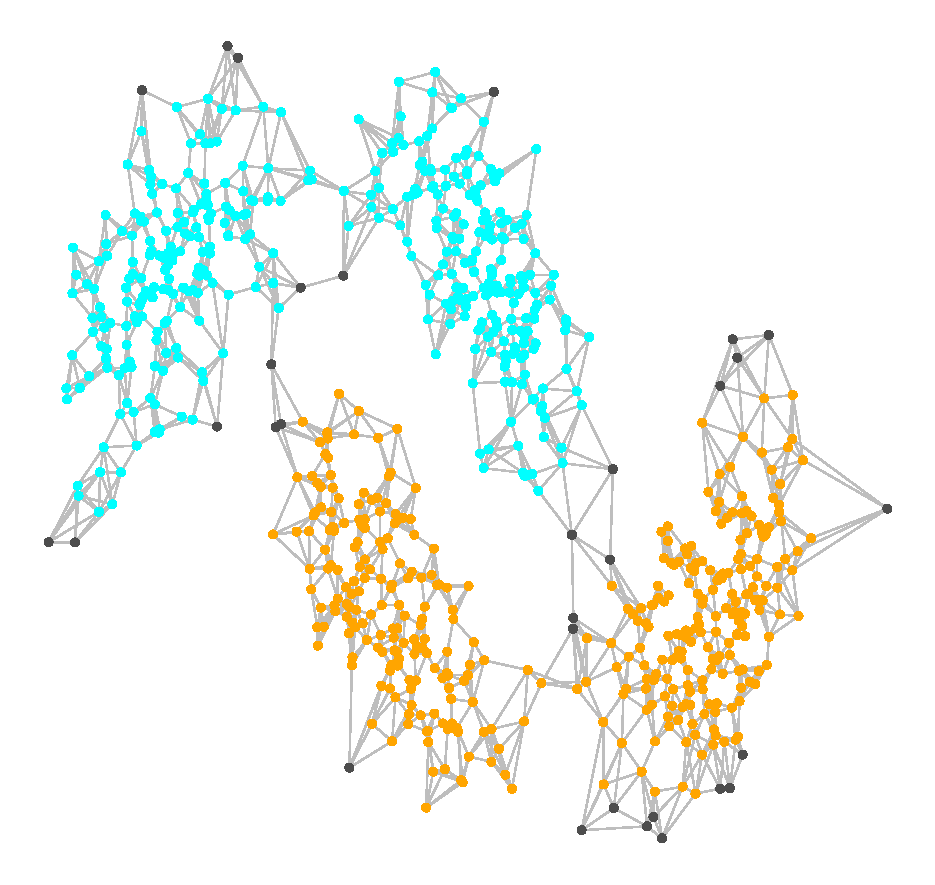
\includegraphics[width=\linewidth,scale = .5]{example3plots/true_density_cluster}
			\caption{}
		\end{subfigure}
		\begin{subfigure}{.24\linewidth}
			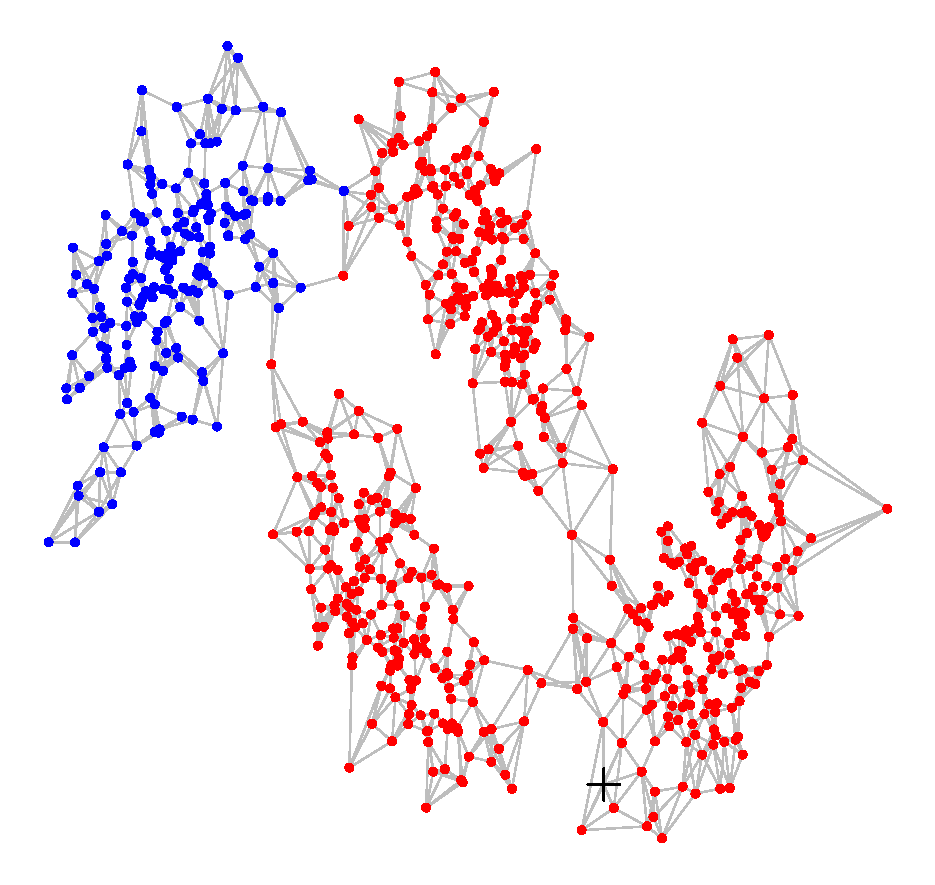
\includegraphics[width=\linewidth,scale = .5]{example3plots/ppr_cluster}
			\caption{}
		\end{subfigure}
		\begin{subfigure}{.24\linewidth}
			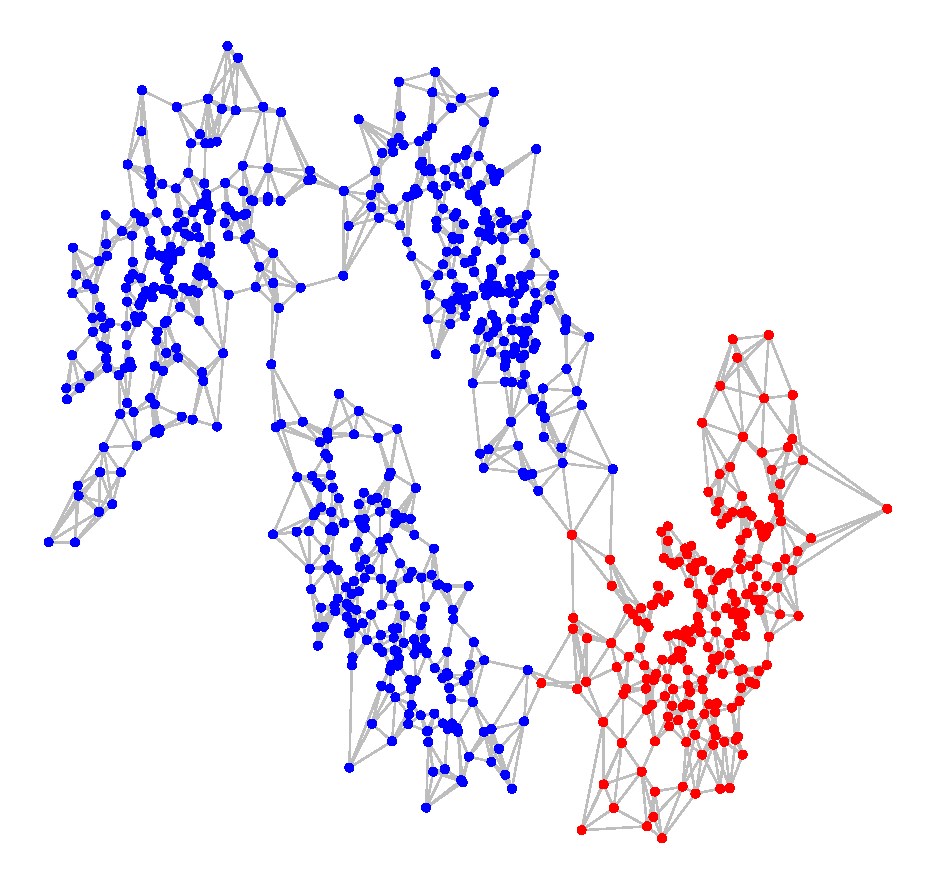
\includegraphics[width=\linewidth,scale = .5]{example3plots/conductance_cluster}
			\caption{}
		\end{subfigure}
		\begin{subfigure}{.24\linewidth}
			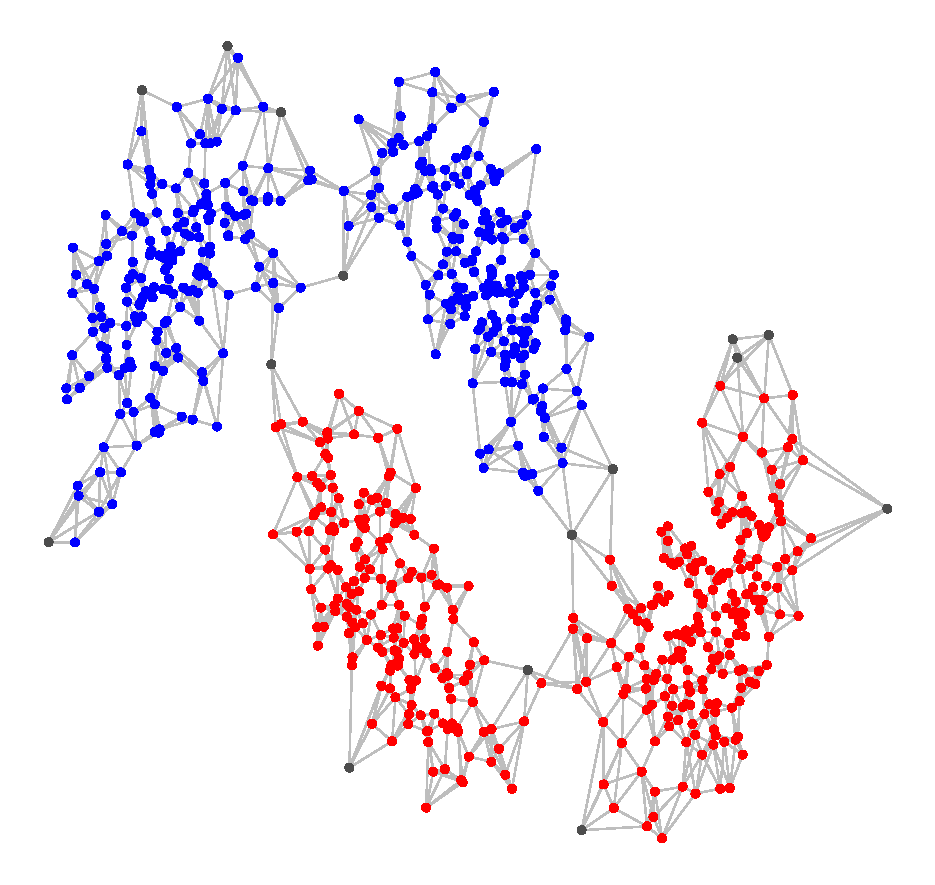
\includegraphics[width=\linewidth,scale = .5]{example3plots/density_cluster}
			\caption{}
		\end{subfigure}
	\caption{}
	\end{adjustbox}
\end{figure}


\section{\textcolor{red}{OLD STUFF}}

\subsection{Volume estimates}
We will fix $\Aset \subset \Rd$ to be an arbitrary set. To simplify expressions, for the $\sigma$-expansion $\Asig$, we will write the set difference between $\Asig$ and the $(\sigma + r)$-expansion $\Aset_{\sigma + r}$ as 
\begin{equation*}
\Asigr := \set{x: 0 < \dist(x, \Asig) \leq r},
\end{equation*}
where as a reminder $\dist(x, \Aset) = \min_{x' \in \Aset} \norm{x - x'}$.

\paragraph{Lemma \ref{lem: interior_of_expansion_sets}.}

We will repeatedly employ Lemma \ref{lem: expansion_sets} and Lemma \ref{lem: Taylor_series} in tandem. As a first example, in Lemma \ref{lem: interior_of_expansion_sets}, we bound the ratio of $\nu(\Aset)$ to $\nu(\Aset_{-\delta})$, where we write $\partial \Aset$ for the boundary of $\Aset$, and for $\delta > 0$ we let
\begin{equation*}
\Aset_{-\delta} : = \set{x \in \Aset: \dist(x, \partial \Aset) > \delta}.
\end{equation*}

This will be useful when we bound $\vol(\Csig)$.

\begin{lemma}
	\label{lem: interior_of_expansion_sets}
	For $\sigma$, $\Asig$ as in Lemma \ref{lem: expansion_sets}, let $r > 0$ satisfy $r \leq \sigma/4d$. Then,
	\begin{equation*}
	\frac{\nu(\Asig)}{\nu(\Aset_{\sigma - r})} \leq 2.
	\end{equation*}
\end{lemma}
\begin{proof}
	Fix $q = \sigma - r$. Then,
	\begin{align*}
	\nu(\Asig) & = \nu(\Aset_{q + \sigma - q}) = \nu(\Aset_q + (\sigma - q)B ) \\
	& \leq \nu(\Aset_q + \frac{(\sigma - q)}{q} \Aset_q) = \left(1 + \frac{\sigma - q}{q}\right)^d \nu(\Aset_q)
	\end{align*}
	where the inequality follows from Lemma \ref{lem: expansion_sets}. Of course, $\sigma - q = r$, and $\frac{r}{q} \leq \frac{1}{2d}$ for $r \leq \frac{1}{4d}$. The claim then follows from Lemma \ref{lem: Taylor_series}.
\end{proof}

\subsection{Proof of Lemma \ref{lem: setup}}

\begin{proof}
	We will write $\Wbf_n = \Dbf_n \Abf_n^{-1}$ for the transition probability matrix over $G_{n,r}$, and let $\widetilde{\Dbf}_n$ and $\widetilde{\Wbf}_n$ be the degree and random walk matrices for the subgraph $\widetilde{G}_{n,r}$.
	
	We introduce \emph{leakage} and \emph{soakage} vectors, defined by
	\begin{align*}
	\ell_t & := e_v (\Wbf_n \widetilde{\mathbf{I}}_n )^t (\mathbf{I}_n - \Dbf_n^{-1} \wDbf_{n}),~ \ell := \sum_{t = 0}^{\infty} (1 - \alpha)^t \ell_t, \\
	s_t & := e_v (\Wbf_n \widetilde{\mathbf{I}}_n )^t (\Wbf_n \widetilde{\mathbf{I}}_n^c),~ s := \sum_{t = 0}^{\infty} (1 - \alpha)^{t} s_t.
	\end{align*}
	where $\mathbf{I}_n$ is the $n \times n$ identity matrix, $\widetilde{\mathbf{I}}_n$ is an $n \times n$ diagonal matrix with $(\widetilde{\mathbf{I}}_n)_{uu} = 1$ if $u \in \Csig[\Xbf]$ and $0$ otherwise, and $\widetilde{\mathbf{I}}_n^c = \mathbf{I}_n - \widetilde{\mathbf{I}}_n$. 
	
	Roughly, the proof of Lemma \ref{lem: setup} will unfold in four steps. The first two will result in the lower bound of (\ref{eqn: lower_bound_PPR_in_cluster}), while the latter two will imply the upper bound in (\ref{eqn: upper_bound_PPR_in_other_cluster}). We briefly summarize the approach before diving into the formal proof:
	
	\begin{enumerate}
		\item For $u \in \Cset[\Xbf]$, we use the results of \cite{zhu2013} to produce the lower bound 
		\begin{equation*}
		\pbf(u) \geq \frac{4}{5}\widetilde{\pi}_{n,r}(u) - \widetilde{\pbf}_{\ell}(u)
		\end{equation*}
		where 
		\begin{equation*}
		\widetilde{\pbf}_{\ell} = \alpha \ell + (1 - \alpha) \widetilde{\pbf}_{\ell} \widetilde{\Wbf}_n
		\end{equation*}
		is the \pprspace random walk over $\widetilde{G}_{n,r}$, and $\ell$ has bounded norm $||\ell||_1 \leq 2\frac{\Phi_{n,r}(\Csig[\Xbf])}{\alpha}$.
		
		\item Since $r < \sigma$, for any $u \in \Cset[\Xbf]$ there are no edges between $u$ and $\Xbf \setminus \Csig[\Xbf]$. Therefore, the page-rank vector $\widetilde{\pbf}_{\ell}$ will not assign more than $||\ell||_1 / d_{\min}(\Csig[\Xbf])$ probability mass to any vertex in $\Cset'[\Xbf]$. This observation will conclude our proof of (\ref{eqn: lower_bound_PPR_in_cluster}).
		\item For vertices $u' \in G_{n,r} / \Csig[\Xbf]$, we can upper bound $p_v(u) \leq p_s(u')$. In particular, this hold for all $u' \in \Cset'[\Xbf]$.
		\item Since $r < \sigma$, there are no edges between $u'$ and $G / \Cset'[\Xbf]$. Therefore, the page-rank vector $p_{s}$ will assign no more than $||s||_1 / d_{\min}(\Csig[\Xbf])$ probability mass to any vertex in $\Cset'[\Xbf]$. Additionally, $s$ has bounded norm $||s||_1 \leq ||\ell||_1$. This will conclude our proof of (\ref{eqn: upper_bound_PPR_in_other_cluster}), and hence Lemma \ref{lem: setup}.
	\end{enumerate}
	
	\paragraph{Step 1}
	We will begin by restating some results of \cite{zhu2013}.
	
	For seed node $v$, we write
	\begin{align} \label{eqn: page_rank_body}
	\widetilde{\pbf}_v & = \alpha e_v + (1 - \alpha) \widetilde{\pbf}_v \widetilde{\Wbf}_n \\
	& = \alpha \sum_{t = 0}^{\infty} (1 - \alpha)^t \left(e_v \widetilde{\Wbf}_n^t \right)
	\end{align}
	
	From Lemma 3.1 of \cite{zhu2013} we have that there exists a good set $\Csig[\Xbf]^g \subseteq \Csig[\Xbf]$ with $\vol(\Csig[\Xbf]^g) \geq \vol(\Csig[\Xbf])/2$ for all $v \in \Csig[\Xbf]^g$, $u \in \Csig[\Xbf]$
	
	\begin{align} \label{eqn: zhu_body}
	p_u & \geq \widetilde{\pbf}_v(u) - \widetilde{\pbf}_{\ell}(u) \nonumber \\
	||\ell||_1 & \leq \frac{2 \widetilde{\Phi}_{n,r}}{\alpha}
	\end{align}
	where $\widetilde{\pbf}_v = (\widetilde{\pbf}_v(u))$ and likewise for $\widetilde{\pbf}_{\ell} = (\widetilde{\pbf}_{\ell}(u))$. (This will be the only time we need to restrict ourselves to this 'good set'.)
	
	Moreover if, as we have specified, $\alpha \leq \widetilde{\Psi}_{n,r}/9$, Lemma 3.2 of \cite{zhu2013} yields a lower bound on $\widetilde{p}$
	\begin{equation} \label{eqn: page_rank_mixes}
	\widetilde{\pbf}_v(u) \geq \frac{4}{5} \widetilde{\pi}_{n,r}(u).
	\end{equation}
	
	\paragraph{Step 2}
	
	We turn to upper bounding $\widetilde{\pbf}_{\ell}(u)$. For any $u \in \Cset[\Xbf]$, we have
	
	\begin{align} \label{eqn: leakage_page_rank_body}
	\widetilde{\pbf}_{\ell}(u) & = \alpha \sum_{t = 0}^{\infty} (1 - \alpha)^t \left(\ell \widetilde{\Wbf}_n^t \right)(u)  \nonumber \\
	& = \|\ell\|_1 \alpha \sum_{t = 0}^{\infty} (1 - \alpha)^t \left(\frac{\ell}{\|\ell\|_1}  \widetilde{\Wbf}_n^t \right)(u)\nonumber \\
	& \overset{\text{(i)}}{=} \|\ell\|_1 \alpha \sum_{t = 1}^{\infty} (1 - \alpha)^t \left(\frac{\ell}{\|\ell\|_1}  \widetilde{\Wbf}_n^t \right)(u)\nonumber \\
	& \overset{\text{(ii)}}{\leq} \|\ell\|_1 \frac{1}{\widetilde{D}_{\min}} 
	\end{align}
	
	where we use $\left(\ell \widetilde{\Wbf}_n^t \right)(u)$ to denote $\ell \widetilde{\Wbf}_n^te_u$.
	
	$\text{(i)}$ follows from the fact that since $r < \sigma$, $\cut(\Cset[\Xbf], G_{n,r} / \Csig[\Xbf]; G_{n,r}) = 0$. Therefore $(\Dbf_n^{-1})_{uu} (\widetilde{\Dbf}_n)_{uu} = 1$, and as a result
	\begin{equation*}
	(\ell \widetilde{\Wbf}_n^0)(u) = \ell(u) = 0.
	\end{equation*}
	To see $\text{(ii)}$, let $q = \frac{\ell}{\|\ell\|_1}  \widetilde{\Wbf}_n^{t-1}$. Then 
	
	\begin{align*}
	\left(\frac{\ell}{\|\ell\|_1}  \widetilde{\Wbf}_n^t \right)(u) & = \left(q \widetilde{\Wbf}_n \right)(u) \\
	& \leq \|q\|_1 \|\widetilde{\Wbf}_{\cdot u}\|_{\infty} \\
	& \overset{\text{(iii)}}{\leq} \frac{1}{\widetilde{D}_{\min}}.
	\end{align*}
	where $\widetilde{\Wbf}_{\cdot u}$ is the $u$th column of $\widetilde{\Wbf}_n$. $\text{(iii)}$ then follows from the fact that any vertex in $\Cset[\Xbf]$ is connected only to vertices in $\Csig[\Xbf]$, and therefore every entry of $\widetilde{\Wbf}_{\cdot u}$ is either $0$ or at most $1 / \widetilde{D}_{\min}$.
	
	
	Combined, (\ref{eqn: leakage_page_rank_body}), (\ref{eqn: page_rank_mixes}), and \eqref{eqn: zhu_body} imply
	\begin{equation*}
	p_v(u) \geq \frac{4}{5} \widetilde{\pi}_{n,r}(u) - 18\frac{ \Phi_{n,r}(\Csig[\Xbf])}{\widetilde{D}_{\min} \alpha}.
	\end{equation*}
	for any $v \in \Csig[\Xbf]$. 
	
	\paragraph{Step 3}
	To get the corresponding upper bound on $p_v(u')$, we will use the soakage vectors $s$ and $s_t$. We will first argue that $s$ is a worse starting distribution -- meaning it puts uniformly more mass outside the cluster -- than simply starting at $v$.
	
	\begin{lemma} \label{lem: gained mass is soaked_body}
		For all $u' \notin \Csig[\Xbf]$,
		\begin{equation}
		\pbf_v(u') \leq \pbf_{s}(u').
		\end{equation}
	\end{lemma}
	
	\begin{proof}
		
		We have
		\begin{align*}
		\pbf_v(u') & = \alpha \sum_{T=0}^{\infty} (1 - \alpha)^T (e_v \Wbf_n^T)(u)\\
		& \overset{(i)}{=} \alpha \sum_{T=1}^{\infty} (1 - \alpha)^T (e_v \Wbf_n^T)(u')
		\end{align*}
		
		where $(i)$ follows from $v \in \Csig$ , $u \not\in \Csig$ and therefore $e_v(u) = 0$. 
		
		Lemma \ref{lem: sum_of_soakages} allows us to make the transition to sums of soakage vectors. 
		\begin{lemma}
			\label{lem: sum_of_soakages}
			
			Let $G = (V,E)$ be a graph, with associated random walk matrix $W$.
			
			For any $T \geq 1$, $q$ vector, $S \subset V$, and $s_t = s_t(S^c,q)$
			\begin{equation}
			qW^T = \sum_{t = 0}^{T - 1} s_t W^{T - t - 1} + q(W I_S)^T
			\end{equation}
		\end{lemma}
		We prove Lemma \ref{lem: sum_of_soakages} after completing the proof of Lemma \ref{lem: gained mass is soaked_body}.
		
		Now, along with the fact $u \not\in \Csig$, we have
		
		\begin{equation*}
		\left(e_v \Wbf_n^T \right)(u') = \sum_{t = 0}^{T - 1} \left(s_t \Wbf_n^{T - t - 1} \right)(u')
		\end{equation*}
		
		and so
		
		\begin{align*}
		\pbf_v(u) & = \alpha \sum_{T=1}^{\infty} (1 - \alpha)^T \left( \sum_{t = 0}^{T - 1} s_t \Wbf^{T - t - 1} \right)(u') \\
		& = \alpha \sum_{t=0}^{\infty} \sum_{T = t + 1}^{\infty} (1 - \alpha)^T \left( s_t \Wbf^{T - t - 1} \right)(u')\\
		& = \alpha \sum_{t=0}^{\infty} \sum_{\Delta = 0}^{\infty} (1 - \alpha)^{\Delta + t + 1} \left( s_t \Wbf_n^{\Delta} \right)(u') \\
		& \leq \alpha \sum_{t=0}^{\infty} \sum_{\Delta = 0}^{\infty} (1 - \alpha)^{\Delta + t } \left( s_t \Wbf_n^{\Delta} \right)(u') \\
		& = \alpha \sum_{\Delta = 0}^{\infty} (1 - \alpha)^{\Delta} \left(s \Wbf_n^{\Delta}\right)(u') \\
		& = \pbf_s(u')
		\end{align*}
	\end{proof}
	
	\begin{proof}[Proof of Lemma \ref{lem: sum_of_soakages}]
		Proceed by induction. When $T = 1$,
		
		\begin{align*}
		qW & = q(WI_S) + q(WI_{S^c}) \\
		& = q(W I_S)^T + s_0 
		\end{align*}
		
		Assume true for $T_0$. For $T = T_0 + 1$,
		
		\begin{align*}
		qW^T & = qW^{T_0}W \\
		& = \left\{ \sum_{t = 0}^{T_0 - 1} s_t W^{T_0 - 1 - t} + q(WI_S)^{T_0} \right\} W \\
		& =  \sum_{t = 0}^{T_0 - 1} s_t W^{T - 1 - t} + q(WI_S)^{T_0}(WI_S + WI_{S^c}) \\
		& =  \sum_{t = 0}^{T - 1} s_t W^{T - 1 - t} + q(WI_S)^{T}
		\end{align*}
	\end{proof}
	
	\paragraph{Step 4}
	
	Just as we upper bounded the probability mass $\widetilde{\pbf}_{\ell}$ could assign to any one vertex, we can upper bound 
	
	\begin{align} \label{eqn: soakage_page_rank_body}
	\pbf_{s}(u') & = \alpha \sum_{t = 0}^{\infty} (1 - \alpha)^t \left(s \Wbf_n^t \right)(u') \nonumber \\
	& = \|s\|_1 \alpha \sum_{t = 0}^{\infty} (1 - \alpha)^t \left(\frac{s}{\|s\|_1} {\Wbf}_n^t \right)(u')\nonumber \\
	& = \|s\|_1 \alpha \sum_{t = 1}^{\infty} (1 - \alpha)^t \left(\frac{s}{\|s\|_1}  {\Wbf}_n^t \right)(u')\nonumber \\
	& \leq \|s\|_1 \frac{1}{\widetilde{D}_{\min}}.
	\end{align}
	
	Finally, letting $q_t = e_v (\Wbf_n \widetilde{\mathbf{I}}_n)^t$ for ease of notation, we have
	\begin{align*}
	\|s_t\|_1 & = \|q_t (\Wbf_n \widetilde{\mathbf{I}}_n)\|_1 \\
	& = \sum_{u' \in \Xbf} \sum_{u \in \Xbf} q_t(u) (\Wbf_n \widetilde{\mathbf{I}}_n)(u, u')\\
	& = \sum_{u' \in \Xbf / \Csig[\Xbf]} \sum_{u \in \Csig[\Xbf]} \frac{q_t(u)}{(\Dbf_n)_{uu}} \1(e_{u,u'} \in G_{n,r}) \\
	& = \sum_{u \in \Csig[\Xbf]} \frac{q(u) \left((\Dbf_n)_{uu} - (\widetilde{\Dbf}_n)_{uu} \right)}{(\Dbf_n)_{uu}} \\
	& = \|q_t (I - \Dbf_n^{-1} \widetilde{\Dbf}_n)\|_1 = \|\ell_t\|_1.
	\end{align*}
	
	and as a result $\|s\|_1 = \|\ell\|_1$. Combining with $\|\ell\|_1 \leq 2 \frac{\widetilde{\Phi}_{n,r}}{\alpha}$ and (\ref{eqn: soakage_page_rank_body}) yields the desired upper bound.
	
\end{proof}

\clearpage
\bibliographystyle{plain}
\bibliography{../local_spectral_bibliography}

\end{document}